\chapter{Higher Order Corrections}
\section{Third Order in e Correction Terms}
Let us first look at a single contraction term in $S^{(3)}$:
\begin{equation}
N \left\{(\linktwoterms{\bar{\psi}}{ \cancel{A} \psi)_{x_{1}}(\bar{\psi}\cancel{A} }{\psi})_{x_{2}}(\bar{\psi}\cancel{A} \psi)_{x_{3}}\right\}
\end{equation}
One of the Feynmann diagrams for this would look like the following figure (\bluep{This is an unconnected diagram, not all lines are connected to one another in a single network})
\begin{figure}[H]
    \centering
\tikzset{every picture/.style={line width=0.75pt}} %set default line width to 0.75pt        

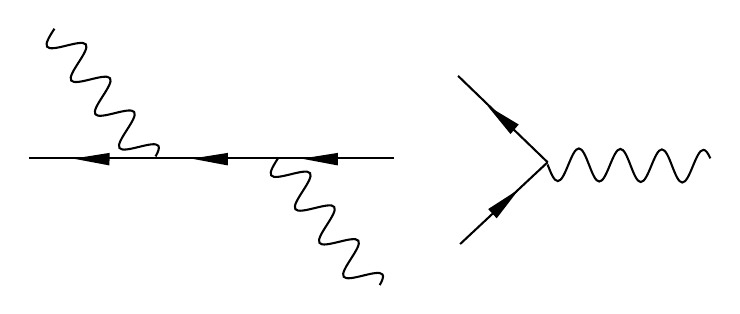
\begin{tikzpicture}[x=0.75pt,y=0.75pt,yscale=-1,xscale=1]
%uncomment if require: \path (0,300); %set diagram left start at 0, and has height of 300

%Straight Lines [id:da3780948069175081] 
\draw    (53,120) -- (228.87,120) ;
%Shape: Triangle [id:dp3960687992590355] 
\draw  [fill={rgb, 255:red, 0; green, 0; blue, 0 }  ,fill opacity=1 ] (134.43,120.3) -- (148.47,118.07) -- (148.4,122.93) -- cycle ;
%Shape: Triangle [id:dp05479485978100629] 
\draw  [fill={rgb, 255:red, 0; green, 0; blue, 0 }  ,fill opacity=1 ] (187.43,120.3) -- (201.47,118.07) -- (201.4,122.93) -- cycle ;
%Shape: Triangle [id:dp7557376074767396] 
\draw  [fill={rgb, 255:red, 0; green, 0; blue, 0 }  ,fill opacity=1 ] (77.43,120.3) -- (91.47,118.07) -- (91.4,122.93) -- cycle ;
%Shape: Wave [id:dp1885622709843502] 
\draw   (65.38,57.66) .. controls (63.03,61.35) and (60.79,64.86) .. (61.85,66.34) .. controls (62.9,67.81) and (66.95,66.83) .. (71.2,65.8) .. controls (75.45,64.76) and (79.5,63.78) .. (80.55,65.25) .. controls (81.61,66.73) and (79.37,70.24) .. (77.02,73.93) .. controls (74.66,77.62) and (72.42,81.13) .. (73.48,82.61) .. controls (74.53,84.08) and (78.58,83.1) .. (82.83,82.07) .. controls (87.08,81.03) and (91.13,80.05) .. (92.19,81.52) .. controls (93.24,83) and (91,86.51) .. (88.65,90.2) .. controls (86.29,93.89) and (84.06,97.4) .. (85.11,98.88) .. controls (86.16,100.35) and (90.21,99.37) .. (94.46,98.34) .. controls (98.71,97.3) and (102.76,96.32) .. (103.82,97.79) .. controls (104.87,99.27) and (102.63,102.78) .. (100.28,106.47) .. controls (97.92,110.16) and (95.69,113.67) .. (96.74,115.15) .. controls (97.79,116.62) and (101.84,115.64) .. (106.09,114.61) .. controls (110.34,113.57) and (114.4,112.59) .. (115.45,114.06) .. controls (116.15,115.05) and (115.39,116.94) .. (114.11,119.18) ;
%Shape: Wave [id:dp8210548245517799] 
\draw   (173.38,119.66) .. controls (171.03,123.35) and (168.79,126.86) .. (169.85,128.34) .. controls (170.9,129.81) and (174.95,128.83) .. (179.2,127.8) .. controls (183.45,126.76) and (187.5,125.78) .. (188.55,127.25) .. controls (189.61,128.73) and (187.37,132.24) .. (185.02,135.93) .. controls (182.66,139.62) and (180.42,143.13) .. (181.48,144.61) .. controls (182.53,146.08) and (186.58,145.1) .. (190.83,144.07) .. controls (195.08,143.03) and (199.13,142.05) .. (200.19,143.52) .. controls (201.24,145) and (199,148.51) .. (196.65,152.2) .. controls (194.29,155.89) and (192.06,159.4) .. (193.11,160.88) .. controls (194.16,162.35) and (198.21,161.37) .. (202.46,160.34) .. controls (206.71,159.3) and (210.76,158.32) .. (211.82,159.79) .. controls (212.87,161.27) and (210.63,164.78) .. (208.28,168.47) .. controls (205.92,172.16) and (203.69,175.67) .. (204.74,177.15) .. controls (205.79,178.62) and (209.84,177.64) .. (214.09,176.61) .. controls (218.34,175.57) and (222.4,174.59) .. (223.45,176.06) .. controls (224.15,177.05) and (223.39,178.94) .. (222.11,181.18) ;
%Straight Lines [id:da5687653686058063] 
\draw    (259.87,80.4) -- (303,122) ;
%Straight Lines [id:da8489603939248399] 
\draw    (303,122) -- (260.87,161.4) ;
%Shape: Triangle [id:dp4508463899972571] 
\draw  [fill={rgb, 255:red, 0; green, 0; blue, 0 }  ,fill opacity=1 ] (276.14,96.63) -- (288.32,103.93) -- (285.14,107.62) -- cycle ;
%Shape: Triangle [id:dp5269520777958134] 
\draw  [fill={rgb, 255:red, 0; green, 0; blue, 0 }  ,fill opacity=1 ] (287.09,136.96) -- (278.43,148.23) -- (275.13,144.65) -- cycle ;
%Shape: Wave [id:dp30185838683938926] 
\draw   (302.99,123.1) .. controls (304.57,127.18) and (306.09,131.06) .. (307.9,131.08) .. controls (309.71,131.1) and (311.31,127.25) .. (312.99,123.21) .. controls (314.66,119.17) and (316.27,115.32) .. (318.08,115.34) .. controls (319.89,115.36) and (321.4,119.25) .. (322.99,123.32) .. controls (324.57,127.4) and (326.09,131.28) .. (327.9,131.3) .. controls (329.71,131.33) and (331.31,127.48) .. (332.99,123.44) .. controls (334.66,119.4) and (336.27,115.55) .. (338.08,115.57) .. controls (339.88,115.59) and (341.4,119.47) .. (342.99,123.55) .. controls (344.57,127.63) and (346.09,131.51) .. (347.89,131.53) .. controls (349.7,131.55) and (351.31,127.71) .. (352.98,123.66) .. controls (354.66,119.62) and (356.26,115.78) .. (358.07,115.8) .. controls (359.88,115.82) and (361.4,119.7) .. (362.98,123.78) .. controls (364.57,127.86) and (366.08,131.74) .. (367.89,131.76) .. controls (369.7,131.78) and (371.31,127.93) .. (372.98,123.89) .. controls (374.66,119.85) and (376.26,116) .. (378.07,116.02) .. controls (379.28,116.04) and (380.36,117.77) .. (381.41,120.13) ;




\end{tikzpicture}
    \caption{Single Contraction term of $S^{(3)}$}
    \label{fig:single-contraction-S3}
\end{figure}
As mentioned in the previous chapter, the single vertex interaction is not physically possible as it produce off-shell photon. We conclude here that \redp{any possible term in $S^{(3)}$ that has a vertex factor $(\bar{\psi}\cancel{A}\psi)_{x_i}$ alone, unconnected to a contraction, is \textbf{not physical and can be ignored.}}

Let's look at one of three contraction term:
\begin{equation}
N \left\{(\UOLunderbr{\bar{\psi} \cancel{A} \overbracket{\psi)_{x_{1}}(\bar{\psi}}}[\cancel{A} \psi]\UOLunderbrl{)_{x_{2}}(\bar{\psi}\cancel{A}} \psi)_{x_{3}}\right\}
\end{equation}
A typical Feynman diagram for this looks like
\begin{figure}[H]
    \centering

\tikzset{every picture/.style={line width=0.75pt}} %set default line width to 0.75pt        

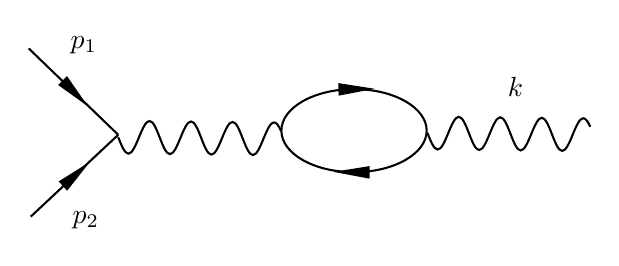
\begin{tikzpicture}[x=0.75pt,y=0.75pt,yscale=-1,xscale=1]
%uncomment if require: \path (0,300); %set diagram left start at 0, and has height of 300

%Straight Lines [id:da5687653686058063] 
\draw    (259.87,80.4) -- (303,122) ;
%Straight Lines [id:da8489603939248399] 
\draw    (303,122) -- (260.87,161.4) ;
%Shape: Triangle [id:dp4508463899972571] 
\draw  [fill={rgb, 255:red, 0; green, 0; blue, 0 }  ,fill opacity=1 ] (287.15,137.03) -- (278.34,148.18) -- (275.1,144.56) -- cycle ;
%Shape: Triangle [id:dp5269520777958134] 
\draw  [fill={rgb, 255:red, 0; green, 0; blue, 0 }  ,fill opacity=1 ] (286.34,106.19) -- (274.79,97.92) -- (278.26,94.5) -- cycle ;
%Shape: Wave [id:dp30185838683938926] 
\draw   (302.99,123.1) .. controls (304.57,127.18) and (306.09,131.06) .. (307.9,131.08) .. controls (309.71,131.1) and (311.31,127.25) .. (312.99,123.21) .. controls (314.66,119.17) and (316.27,115.32) .. (318.08,115.34) .. controls (319.89,115.36) and (321.4,119.25) .. (322.99,123.32) .. controls (324.57,127.4) and (326.09,131.28) .. (327.9,131.3) .. controls (329.71,131.33) and (331.31,127.48) .. (332.99,123.44) .. controls (334.66,119.4) and (336.27,115.55) .. (338.08,115.57) .. controls (339.88,115.59) and (341.4,119.47) .. (342.99,123.55) .. controls (344.57,127.63) and (346.09,131.51) .. (347.89,131.53) .. controls (349.7,131.55) and (351.31,127.71) .. (352.98,123.66) .. controls (354.66,119.62) and (356.26,115.78) .. (358.07,115.8) .. controls (359.88,115.82) and (361.4,119.7) .. (362.98,123.78) .. controls (364.57,127.86) and (366.08,131.74) .. (367.89,131.76) .. controls (369.7,131.78) and (371.31,127.93) .. (372.98,123.89) .. controls (374.66,119.85) and (376.26,116) .. (378.07,116.02) .. controls (379.28,116.04) and (380.36,117.77) .. (381.41,120.13) ;
%Shape: Ellipse [id:dp21378260759473022] 
\draw   (381.6,120) .. controls (381.6,108.95) and (397.27,100) .. (416.6,100) .. controls (435.93,100) and (451.6,108.95) .. (451.6,120) .. controls (451.6,131.05) and (435.93,140) .. (416.6,140) .. controls (397.27,140) and (381.6,131.05) .. (381.6,120) -- cycle ;
%Shape: Wave [id:dp07427295068477802] 
\draw   (451.99,121.1) .. controls (453.57,125.18) and (455.09,129.06) .. (456.9,129.08) .. controls (458.71,129.1) and (460.31,125.25) .. (461.99,121.21) .. controls (463.66,117.17) and (465.27,113.32) .. (467.08,113.34) .. controls (468.89,113.36) and (470.4,117.25) .. (471.99,121.32) .. controls (473.57,125.4) and (475.09,129.28) .. (476.9,129.3) .. controls (478.71,129.33) and (480.31,125.48) .. (481.99,121.44) .. controls (483.66,117.4) and (485.27,113.55) .. (487.08,113.57) .. controls (488.88,113.59) and (490.4,117.47) .. (491.99,121.55) .. controls (493.57,125.63) and (495.09,129.51) .. (496.89,129.53) .. controls (498.7,129.55) and (500.31,125.71) .. (501.98,121.66) .. controls (503.66,117.62) and (505.26,113.78) .. (507.07,113.8) .. controls (508.88,113.82) and (510.4,117.7) .. (511.98,121.78) .. controls (513.57,125.86) and (515.08,129.74) .. (516.89,129.76) .. controls (518.7,129.78) and (520.31,125.93) .. (521.98,121.89) .. controls (523.66,117.85) and (525.26,114) .. (527.07,114.02) .. controls (528.28,114.04) and (529.36,115.77) .. (530.41,118.13) ;
%Shape: Triangle [id:dp13296502270667654] 
\draw  [fill={rgb, 255:red, 0; green, 0; blue, 0 }  ,fill opacity=1 ] (409.6,139.9) -- (423.63,137.67) -- (423.56,142.53) -- cycle ;
%Shape: Triangle [id:dp9482730045827157] 
\draw  [fill={rgb, 255:red, 0; green, 0; blue, 0 }  ,fill opacity=1 ] (423.6,99.88) -- (409.64,102.55) -- (409.56,97.68) -- cycle ;

% Text Node
\draw (286.4,79) node    {$p_{1}$};
% Text Node
\draw (287.4,163) node    {$p_{2}$};
% Text Node
\draw (494.4,99) node    {$k$};


\end{tikzpicture}
    \caption{A Three Contraction Term of $S^{(3)}$}
    \label{fig:3-contraction-S3}
\end{figure}
Note that the net result of Fig.(\ref{fig:3-contraction-S3}) is similar to what we saw in the previous chapter, where a real electron and a real positron transmute into a single off-shell photon. Thus, it is unphysical too.
\begin{center}
    \tikzset{every picture/.style={line width=0.75pt}} %set default line width to 0.75pt 
\begin{tikzpicture}[x=0.75pt,y=0.75pt,yscale=-1,xscale=1]
%uncomment if require: \path (0,300); %set diagram left start at 0, and has height of 300

%Straight Lines [id:da307650809518932] 
\draw    (58,58.37) -- (158,158.37) ;
%Straight Lines [id:da4053696323117585] 
\draw    (158,158.37) -- (59.87,247.8) ;
%Shape: Wave [id:dp5998613246245391] 
\draw   (158,157.8) .. controls (162.14,161.39) and (166.11,164.8) .. (170.63,164.8) .. controls (175.16,164.8) and (178.99,161.39) .. (183,157.8) .. controls (187.01,154.21) and (190.84,150.8) .. (195.37,150.8) .. controls (199.89,150.8) and (203.85,154.21) .. (208,157.8) .. controls (212.14,161.39) and (216.11,164.8) .. (220.63,164.8) .. controls (225.16,164.8) and (228.99,161.39) .. (233,157.8) .. controls (237.01,154.21) and (240.84,150.8) .. (245.37,150.8) .. controls (249.89,150.8) and (253.85,154.21) .. (258,157.8) .. controls (262.14,161.39) and (266.11,164.8) .. (270.63,164.8) .. controls (275.16,164.8) and (278.99,161.39) .. (283,157.8) .. controls (287.01,154.21) and (290.84,150.8) .. (295.37,150.8) .. controls (299.89,150.8) and (303.85,154.21) .. (308,157.8) .. controls (312.14,161.39) and (316.11,164.8) .. (320.63,164.8) .. controls (325.16,164.8) and (328.99,161.39) .. (333,157.8) .. controls (333,157.8) and (333,157.8) .. (333,157.8) ;
%Shape: Triangle [id:dp4766081790625024] 
\draw  [fill={rgb, 255:red, 0; green, 0; blue, 0 }  ,fill opacity=1 ] (115.33,115.49) -- (97.69,104.32) -- (103.66,98.17) -- cycle ;
%Shape: Triangle [id:dp2439506934283957] 
\draw  [fill={rgb, 255:red, 0; green, 0; blue, 0 }  ,fill opacity=1 ] (101.73,210.33) -- (113.1,192.82) -- (119.17,198.86) -- cycle ;

% Text Node
\draw (86,61.37) node    {$p_{1}$};
% Text Node
\draw (88,244.37) node    {$p_{2}$};
% Text Node
\draw (256,134.37) node    {$k$};


\end{tikzpicture}
\end{center}
In similar fashion, we can show that \redp{every term in $S^{(3)}$ is unphysical and contributes zero to the transmission amplitude.}

\begin{qt}
    Feynman's rules ignore the factorial in the denominator of each term because those rules are applied to each topologically distinct diagram.
\end{qt}
\section{Fourth Order in e Correction Terms}
The $e^4$ order contributions to 1st kind of Bhabha scattering is shown in the following figure:
\begin{figure}[H]
    \centering
\tikzset{every picture/.style={line width=0.75pt}} %set default line width to 0.75pt        
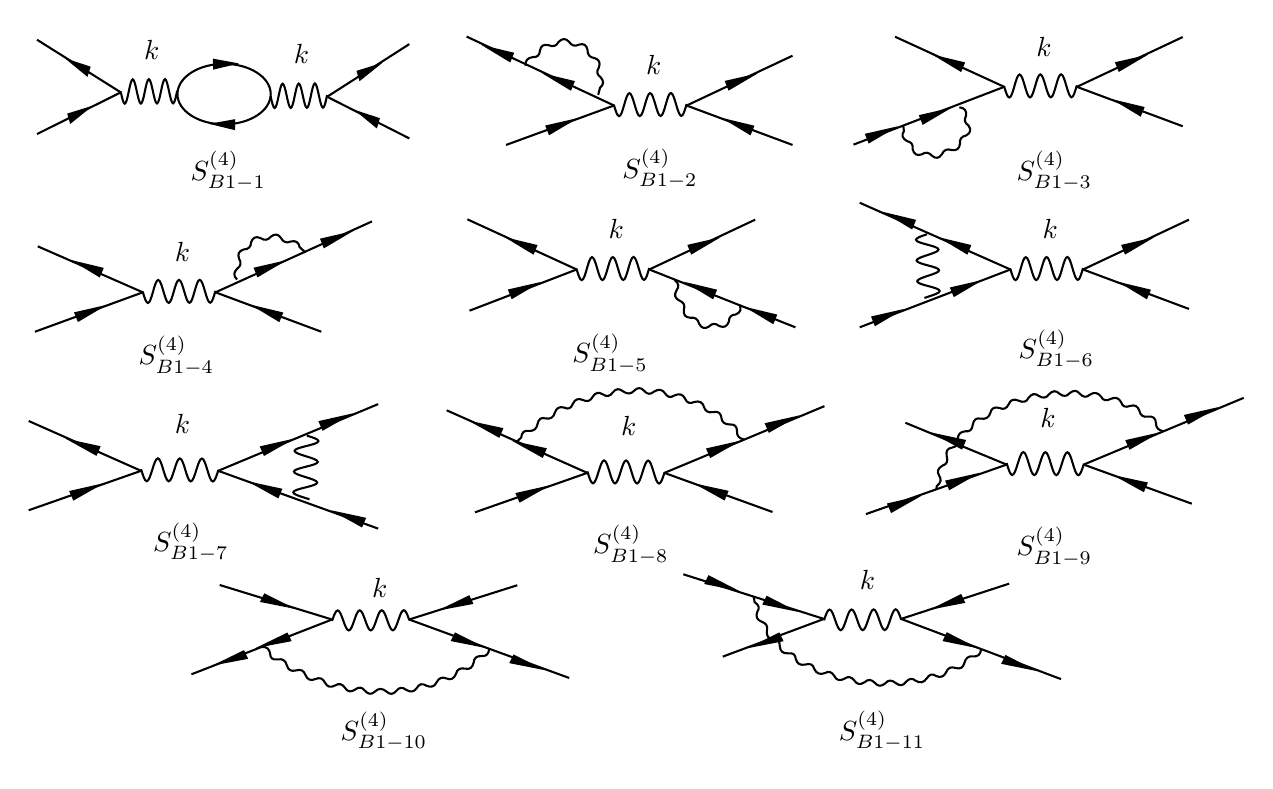
\begin{tikzpicture}[x=0.75pt,y=0.75pt,yscale=-1,xscale=1]
%uncomment if require: \path (0,373); %set diagram left start at 0, and has height of 373

%Straight Lines [id:da011089109916939899] 
\draw    (50.87,20.74) -- (91.25,46.1) ;
%Straight Lines [id:da43361859076573783] 
\draw    (91.25,46.1) -- (50.87,66.17) ;
%Shape: Wave [id:dp561316452516215] 
\draw   (91.19,45.69) .. controls (91.83,48.68) and (92.44,51.52) .. (93.14,51.52) .. controls (93.85,51.51) and (94.44,48.66) .. (95.07,45.67) .. controls (95.69,42.68) and (96.29,39.83) .. (96.99,39.82) .. controls (97.69,39.82) and (98.31,42.66) .. (98.95,45.65) .. controls (99.59,48.63) and (100.21,51.48) .. (100.91,51.47) .. controls (101.61,51.47) and (102.21,48.62) .. (102.83,45.63) .. controls (103.46,42.63) and (104.05,39.78) .. (104.76,39.78) .. controls (105.46,39.78) and (106.07,42.62) .. (106.72,45.61) .. controls (107.36,48.59) and (107.97,51.44) .. (108.67,51.43) .. controls (109.38,51.43) and (109.97,48.58) .. (110.6,45.59) .. controls (111.22,42.59) and (111.82,39.74) .. (112.52,39.74) .. controls (113.23,39.73) and (113.84,42.58) .. (114.48,45.56) .. controls (115.12,48.55) and (115.74,51.39) .. (116.44,51.39) .. controls (117.14,51.39) and (117.74,48.54) .. (118.36,45.54) .. controls (118.38,45.47) and (118.39,45.4) .. (118.41,45.33) ;
%Shape: Ellipse [id:dp9186385161248081] 
\draw   (118.53,46.92) .. controls (118.53,38.88) and (128.59,32.36) .. (141,32.36) .. controls (153.41,32.36) and (163.47,38.88) .. (163.47,46.92) .. controls (163.47,54.97) and (153.41,61.49) .. (141,61.49) .. controls (128.59,61.49) and (118.53,54.97) .. (118.53,46.92) -- cycle ;
%Shape: Wave [id:dp39272359818025504] 
\draw   (163.4,47.8) .. controls (164.05,50.79) and (164.66,53.63) .. (165.36,53.63) .. controls (166.07,53.63) and (166.66,50.78) .. (167.29,47.78) .. controls (167.91,44.79) and (168.51,41.94) .. (169.21,41.94) .. controls (169.91,41.93) and (170.53,44.78) .. (171.17,47.76) .. controls (171.81,50.75) and (172.43,53.59) .. (173.13,53.59) .. controls (173.83,53.58) and (174.43,50.73) .. (175.05,47.74) .. controls (175.68,44.75) and (176.27,41.9) .. (176.98,41.89) .. controls (177.68,41.89) and (178.29,44.73) .. (178.94,47.72) .. controls (179.58,50.71) and (180.19,53.55) .. (180.89,53.54) .. controls (181.6,53.54) and (182.19,50.69) .. (182.82,47.7) .. controls (183.44,44.71) and (184.04,41.86) .. (184.74,41.85) .. controls (185.44,41.85) and (186.06,44.69) .. (186.7,47.68) .. controls (187.34,50.66) and (187.96,53.51) .. (188.66,53.5) .. controls (189.36,53.5) and (189.96,50.65) .. (190.58,47.66) .. controls (190.6,47.58) and (190.61,47.51) .. (190.63,47.44) ;
%Straight Lines [id:da5365655317348891] 
\draw    (230.25,22.85) -- (190.65,48.21) ;
%Straight Lines [id:da3871952851348154] 
\draw    (190.65,48.21) -- (230.25,68.28) ;
%Shape: Triangle [id:dp6412237399505359] 
\draw  [fill={rgb, 255:red, 0; green, 0; blue, 0 }  ,fill opacity=1 ] (66.59,30.92) -- (76.09,34.03) -- (74.95,37.8) -- cycle ;
%Shape: Triangle [id:dp6791473471754387] 
\draw  [fill={rgb, 255:red, 0; green, 0; blue, 0 }  ,fill opacity=1 ] (205.98,55.75) -- (215.48,58.85) -- (214.34,62.63) -- cycle ;
%Shape: Triangle [id:dp06307672956548438] 
\draw  [fill={rgb, 255:red, 0; green, 0; blue, 0 }  ,fill opacity=1 ] (75.54,53.71) -- (67.13,60.46) -- (66.02,56.66) -- cycle ;
%Shape: Triangle [id:dp3796807271349131] 
\draw  [fill={rgb, 255:red, 0; green, 0; blue, 0 }  ,fill opacity=1 ] (214.93,33.1) -- (206.52,39.86) -- (205.41,36.06) -- cycle ;
%Shape: Triangle [id:dp443230832318676] 
\draw  [fill={rgb, 255:red, 0; green, 0; blue, 0 }  ,fill opacity=1 ] (145.82,32.23) -- (136.2,34.53) -- (136.14,30.45) -- cycle ;
%Shape: Triangle [id:dp16213431943034184] 
\draw  [fill={rgb, 255:red, 0; green, 0; blue, 0 }  ,fill opacity=1 ] (136.17,61.34) -- (145.86,59.59) -- (145.79,63.67) -- cycle ;
%Straight Lines [id:da8617687990925555] 
\draw    (257.87,19.23) -- (328.87,52.43) ;
%Straight Lines [id:da9328000627888356] 
\draw    (328.87,52.43) -- (276.87,71.43) ;
%Shape: Wave [id:dp8163789548492385] 
\draw   (328.79,52.05) .. controls (329.61,54.88) and (330.4,57.57) .. (331.31,57.56) .. controls (332.21,57.56) and (332.98,54.86) .. (333.79,52.03) .. controls (334.59,49.2) and (335.36,46.5) .. (336.26,46.49) .. controls (337.17,46.49) and (337.96,49.18) .. (338.79,52.01) .. controls (339.61,54.84) and (340.4,57.53) .. (341.31,57.52) .. controls (342.21,57.52) and (342.98,54.82) .. (343.79,51.99) .. controls (344.59,49.16) and (345.36,46.46) .. (346.26,46.45) .. controls (347.17,46.45) and (347.96,49.14) .. (348.79,51.97) .. controls (349.61,54.8) and (350.4,57.49) .. (351.31,57.48) .. controls (352.21,57.48) and (352.98,54.78) .. (353.79,51.95) .. controls (354.59,49.12) and (355.36,46.42) .. (356.26,46.41) .. controls (357.17,46.41) and (357.96,49.1) .. (358.79,51.93) .. controls (359.61,54.76) and (360.4,57.45) .. (361.31,57.44) .. controls (362.21,57.44) and (362.98,54.74) .. (363.79,51.91) .. controls (363.81,51.84) and (363.82,51.77) .. (363.84,51.71) ;
%Straight Lines [id:da33216942396714977] 
\draw    (414.87,28.43) -- (363.87,52.43) ;
%Straight Lines [id:da2656267933846157] 
\draw    (363.87,52.43) -- (414.87,71.43) ;
%Shape: Triangle [id:dp8942845965075189] 
\draw  [fill={rgb, 255:red, 0; green, 0; blue, 0 }  ,fill opacity=1 ] (297.12,38.07) -- (309.35,41.01) -- (307.88,44.58) -- cycle ;
%Shape: Triangle [id:dp6157826595985776] 
\draw  [fill={rgb, 255:red, 0; green, 0; blue, 0 }  ,fill opacity=1 ] (383.62,59.57) -- (395.85,62.51) -- (394.38,66.08) -- cycle ;
%Shape: Triangle [id:dp641401913429291] 
\draw  [fill={rgb, 255:red, 0; green, 0; blue, 0 }  ,fill opacity=1 ] (308.64,59.63) -- (297.81,66.03) -- (296.38,62.44) -- cycle ;
%Shape: Triangle [id:dp4350046220043283] 
\draw  [fill={rgb, 255:red, 0; green, 0; blue, 0 }  ,fill opacity=1 ] (395.14,38.13) -- (384.31,44.53) -- (382.88,40.94) -- cycle ;
%Shape: Triangle [id:dp34063851978227133] 
\draw  [fill={rgb, 255:red, 0; green, 0; blue, 0 }  ,fill opacity=1 ] (267.87,24.43) -- (280.1,27.37) -- (278.63,30.95) -- cycle ;
%Straight Lines [id:da3363460034806529] 
\draw    (464.25,19.28) -- (516.87,43.43) ;
%Straight Lines [id:da7611083532520225] 
\draw    (516.87,43.43) -- (444.25,71.28) ;
%Shape: Wave [id:dp7086964369596943] 
\draw   (516.79,43.05) .. controls (517.61,45.88) and (518.4,48.57) .. (519.31,48.56) .. controls (520.21,48.56) and (520.98,45.86) .. (521.79,43.03) .. controls (522.59,40.2) and (523.36,37.5) .. (524.26,37.49) .. controls (525.17,37.49) and (525.96,40.18) .. (526.79,43.01) .. controls (527.61,45.84) and (528.4,48.53) .. (529.31,48.52) .. controls (530.21,48.52) and (530.98,45.82) .. (531.79,42.99) .. controls (532.59,40.16) and (533.36,37.46) .. (534.26,37.45) .. controls (535.17,37.45) and (535.96,40.14) .. (536.79,42.97) .. controls (537.61,45.8) and (538.4,48.49) .. (539.31,48.48) .. controls (540.21,48.48) and (540.98,45.78) .. (541.79,42.95) .. controls (542.59,40.12) and (543.36,37.42) .. (544.26,37.41) .. controls (545.17,37.41) and (545.96,40.1) .. (546.79,42.93) .. controls (547.61,45.76) and (548.4,48.45) .. (549.31,48.44) .. controls (550.21,48.44) and (550.98,45.74) .. (551.79,42.91) .. controls (551.81,42.84) and (551.82,42.77) .. (551.84,42.71) ;
%Straight Lines [id:da32782854414498586] 
\draw    (602.87,19.43) -- (551.87,43.43) ;
%Straight Lines [id:da9757141946780049] 
\draw    (551.87,43.43) -- (602.87,62.43) ;
%Shape: Triangle [id:dp8050538717551093] 
\draw  [fill={rgb, 255:red, 0; green, 0; blue, 0 }  ,fill opacity=1 ] (485.12,29.07) -- (497.35,32.01) -- (495.88,35.58) -- cycle ;
%Shape: Triangle [id:dp550943935919394] 
\draw  [fill={rgb, 255:red, 0; green, 0; blue, 0 }  ,fill opacity=1 ] (571.62,50.57) -- (583.85,53.51) -- (582.38,57.08) -- cycle ;
%Shape: Triangle [id:dp3552152886617791] 
\draw  [fill={rgb, 255:red, 0; green, 0; blue, 0 }  ,fill opacity=1 ] (488.64,54.63) -- (477.81,61.03) -- (476.38,57.44) -- cycle ;
%Shape: Triangle [id:dp08529281861249294] 
\draw  [fill={rgb, 255:red, 0; green, 0; blue, 0 }  ,fill opacity=1 ] (583.14,29.13) -- (572.31,35.53) -- (570.88,31.94) -- cycle ;
%Shape: Triangle [id:dp8688636547126236] 
\draw  [fill={rgb, 255:red, 0; green, 0; blue, 0 }  ,fill opacity=1 ] (462.64,63.63) -- (451.81,70.03) -- (450.38,66.44) -- cycle ;
%Straight Lines [id:da7494274527821663] 
\draw    (51.25,120.28) -- (101.87,142.43) ;
%Straight Lines [id:da4087104776756034] 
\draw    (101.87,142.43) -- (49.87,161.43) ;
%Shape: Wave [id:dp7937084762228351] 
\draw   (101.79,142.05) .. controls (102.61,144.88) and (103.4,147.57) .. (104.31,147.56) .. controls (105.21,147.56) and (105.98,144.86) .. (106.79,142.03) .. controls (107.59,139.2) and (108.36,136.5) .. (109.26,136.49) .. controls (110.17,136.49) and (110.96,139.18) .. (111.79,142.01) .. controls (112.61,144.84) and (113.4,147.53) .. (114.31,147.52) .. controls (115.21,147.52) and (115.98,144.82) .. (116.79,141.99) .. controls (117.59,139.16) and (118.36,136.46) .. (119.26,136.45) .. controls (120.17,136.45) and (120.96,139.14) .. (121.79,141.97) .. controls (122.61,144.8) and (123.4,147.49) .. (124.31,147.48) .. controls (125.21,147.48) and (125.98,144.78) .. (126.79,141.95) .. controls (127.59,139.12) and (128.36,136.42) .. (129.26,136.41) .. controls (130.17,136.41) and (130.96,139.1) .. (131.79,141.93) .. controls (132.61,144.76) and (133.4,147.45) .. (134.31,147.44) .. controls (135.21,147.44) and (135.98,144.74) .. (136.79,141.91) .. controls (136.81,141.84) and (136.82,141.77) .. (136.84,141.71) ;
%Straight Lines [id:da3596469877108829] 
\draw    (212.25,108.28) -- (136.87,142.43) ;
%Straight Lines [id:da5080962588439405] 
\draw    (136.87,142.43) -- (187.87,161.43) ;
%Shape: Triangle [id:dp4945561919496638] 
\draw  [fill={rgb, 255:red, 0; green, 0; blue, 0 }  ,fill opacity=1 ] (70.12,128.07) -- (82.35,131.01) -- (80.88,134.58) -- cycle ;
%Shape: Triangle [id:dp6373274627188662] 
\draw  [fill={rgb, 255:red, 0; green, 0; blue, 0 }  ,fill opacity=1 ] (156.62,149.57) -- (168.85,152.51) -- (167.38,156.08) -- cycle ;
%Shape: Triangle [id:dp3622411241034931] 
\draw  [fill={rgb, 255:red, 0; green, 0; blue, 0 }  ,fill opacity=1 ] (81.64,149.63) -- (70.81,156.03) -- (69.38,152.44) -- cycle ;
%Shape: Triangle [id:dp9730988923754403] 
\draw  [fill={rgb, 255:red, 0; green, 0; blue, 0 }  ,fill opacity=1 ] (168.14,128.13) -- (157.31,134.53) -- (155.88,130.94) -- cycle ;
%Shape: Triangle [id:dp9290869770177214] 
\draw  [fill={rgb, 255:red, 0; green, 0; blue, 0 }  ,fill opacity=1 ] (200.14,114.13) -- (189.31,120.53) -- (187.88,116.94) -- cycle ;
%Straight Lines [id:da20444234472642975] 
\draw    (258.25,107.28) -- (310.87,131.43) ;
%Straight Lines [id:da7426776623630428] 
\draw    (310.87,131.43) -- (259.25,151.28) ;
%Shape: Wave [id:dp3391526165310703] 
\draw   (310.79,131.05) .. controls (311.61,133.88) and (312.4,136.57) .. (313.31,136.56) .. controls (314.21,136.56) and (314.98,133.86) .. (315.79,131.03) .. controls (316.59,128.2) and (317.36,125.5) .. (318.26,125.49) .. controls (319.17,125.49) and (319.96,128.18) .. (320.79,131.01) .. controls (321.61,133.84) and (322.4,136.53) .. (323.31,136.52) .. controls (324.21,136.52) and (324.98,133.82) .. (325.79,130.99) .. controls (326.59,128.16) and (327.36,125.46) .. (328.26,125.45) .. controls (329.17,125.45) and (329.96,128.14) .. (330.79,130.97) .. controls (331.61,133.8) and (332.4,136.49) .. (333.31,136.48) .. controls (334.21,136.48) and (334.98,133.78) .. (335.79,130.95) .. controls (336.59,128.12) and (337.36,125.42) .. (338.26,125.41) .. controls (339.17,125.41) and (339.96,128.1) .. (340.79,130.93) .. controls (341.61,133.76) and (342.4,136.45) .. (343.31,136.44) .. controls (344.21,136.44) and (344.98,133.74) .. (345.79,130.91) .. controls (345.81,130.84) and (345.82,130.77) .. (345.84,130.71) ;
%Straight Lines [id:da8792801927098088] 
\draw    (396.87,107.43) -- (345.87,131.43) ;
%Straight Lines [id:da9070065394777989] 
\draw    (345.87,131.43) -- (416.25,159.28) ;
%Shape: Triangle [id:dp9166509667715766] 
\draw  [fill={rgb, 255:red, 0; green, 0; blue, 0 }  ,fill opacity=1 ] (279.12,117.07) -- (291.35,120.01) -- (289.88,123.58) -- cycle ;
%Shape: Triangle [id:dp6947654293165709] 
\draw  [fill={rgb, 255:red, 0; green, 0; blue, 0 }  ,fill opacity=1 ] (365.62,138.57) -- (377.85,141.51) -- (376.38,145.08) -- cycle ;
%Shape: Triangle [id:dp1369263403546639] 
\draw  [fill={rgb, 255:red, 0; green, 0; blue, 0 }  ,fill opacity=1 ] (290.64,138.63) -- (279.81,145.03) -- (278.38,141.44) -- cycle ;
%Shape: Triangle [id:dp03775848002064475] 
\draw  [fill={rgb, 255:red, 0; green, 0; blue, 0 }  ,fill opacity=1 ] (377.14,117.13) -- (366.31,123.53) -- (364.88,119.94) -- cycle ;
%Shape: Triangle [id:dp9148195160286381] 
\draw  [fill={rgb, 255:red, 0; green, 0; blue, 0 }  ,fill opacity=1 ] (394.62,150.57) -- (406.85,153.51) -- (405.38,157.08) -- cycle ;
%Straight Lines [id:da8604105876253021] 
\draw    (447.25,99.28) -- (519.87,131.43) ;
%Straight Lines [id:da2782340961497919] 
\draw    (519.87,131.43) -- (447.25,159.28) ;
%Shape: Wave [id:dp7846293714759067] 
\draw   (519.79,131.05) .. controls (520.61,133.88) and (521.4,136.57) .. (522.31,136.56) .. controls (523.21,136.56) and (523.98,133.86) .. (524.79,131.03) .. controls (525.59,128.2) and (526.36,125.5) .. (527.26,125.49) .. controls (528.17,125.49) and (528.96,128.18) .. (529.79,131.01) .. controls (530.61,133.84) and (531.4,136.53) .. (532.31,136.52) .. controls (533.21,136.52) and (533.98,133.82) .. (534.79,130.99) .. controls (535.59,128.16) and (536.36,125.46) .. (537.26,125.45) .. controls (538.17,125.45) and (538.96,128.14) .. (539.79,130.97) .. controls (540.61,133.8) and (541.4,136.49) .. (542.31,136.48) .. controls (543.21,136.48) and (543.98,133.78) .. (544.79,130.95) .. controls (545.59,128.12) and (546.36,125.42) .. (547.26,125.41) .. controls (548.17,125.41) and (548.96,128.1) .. (549.79,130.93) .. controls (550.61,133.76) and (551.4,136.45) .. (552.31,136.44) .. controls (553.21,136.44) and (553.98,133.74) .. (554.79,130.91) .. controls (554.81,130.84) and (554.82,130.77) .. (554.84,130.71) ;
%Straight Lines [id:da24662017466488517] 
\draw    (605.87,107.43) -- (554.87,131.43) ;
%Straight Lines [id:da7471294883249145] 
\draw    (554.87,131.43) -- (605.87,150.43) ;
%Shape: Triangle [id:dp5376496958855946] 
\draw  [fill={rgb, 255:red, 0; green, 0; blue, 0 }  ,fill opacity=1 ] (488.12,117.07) -- (500.35,120.01) -- (498.88,123.58) -- cycle ;
%Shape: Triangle [id:dp4602196040872505] 
\draw  [fill={rgb, 255:red, 0; green, 0; blue, 0 }  ,fill opacity=1 ] (574.62,138.57) -- (586.85,141.51) -- (585.38,145.08) -- cycle ;
%Shape: Triangle [id:dp47021354498241397] 
\draw  [fill={rgb, 255:red, 0; green, 0; blue, 0 }  ,fill opacity=1 ] (503.64,137.63) -- (492.81,144.03) -- (491.38,140.44) -- cycle ;
%Shape: Triangle [id:dp9030198894599027] 
\draw  [fill={rgb, 255:red, 0; green, 0; blue, 0 }  ,fill opacity=1 ] (586.14,117.13) -- (575.31,123.53) -- (573.88,119.94) -- cycle ;
%Shape: Triangle [id:dp07541784138123875] 
\draw  [fill={rgb, 255:red, 0; green, 0; blue, 0 }  ,fill opacity=1 ] (465.64,151.63) -- (454.81,158.03) -- (453.38,154.44) -- cycle ;
%Shape: Triangle [id:dp8523536990555651] 
\draw  [fill={rgb, 255:red, 0; green, 0; blue, 0 }  ,fill opacity=1 ] (461.5,104.92) -- (473.73,107.86) -- (472.27,111.43) -- cycle ;
%Shape: Wave [id:dp9224365565152917] 
\draw   (479.64,114.46) .. controls (476.92,115.36) and (474.34,116.21) .. (474.36,117.11) .. controls (474.39,118.02) and (477.02,118.72) .. (479.78,119.46) .. controls (482.55,120.2) and (485.18,120.9) .. (485.2,121.81) .. controls (485.23,122.71) and (482.64,123.56) .. (479.93,124.46) .. controls (477.21,125.35) and (474.62,126.21) .. (474.65,127.11) .. controls (474.68,128.01) and (477.31,128.72) .. (480.07,129.46) .. controls (482.83,130.19) and (485.46,130.9) .. (485.49,131.8) .. controls (485.52,132.71) and (482.93,133.56) .. (480.21,134.45) .. controls (477.5,135.35) and (474.91,136.2) .. (474.94,137.11) .. controls (474.96,138.01) and (477.59,138.72) .. (480.36,139.45) .. controls (483.12,140.19) and (485.75,140.89) .. (485.78,141.8) .. controls (485.8,142.7) and (483.22,143.56) .. (480.5,144.45) .. controls (479.79,144.68) and (479.08,144.92) .. (478.43,145.15) ;
%Straight Lines [id:da6129594130571486] 
\draw    (215.25,196.28) -- (138.16,228.43) ;
%Straight Lines [id:da8285292168968681] 
\draw    (138.16,228.43) -- (215.25,256.28) ;
%Shape: Wave [id:dp3867433749303837] 
\draw   (138.25,228.05) .. controls (137.37,230.88) and (136.53,233.57) .. (135.57,233.56) .. controls (134.61,233.56) and (133.79,230.86) .. (132.94,228.03) .. controls (132.09,225.2) and (131.27,222.5) .. (130.31,222.5) .. controls (129.35,222.49) and (128.51,225.18) .. (127.63,228.01) .. controls (126.75,230.84) and (125.91,233.53) .. (124.95,233.52) .. controls (123.99,233.52) and (123.18,230.82) .. (122.32,227.99) .. controls (121.47,225.16) and (120.65,222.46) .. (119.69,222.46) .. controls (118.73,222.45) and (117.89,225.14) .. (117.02,227.97) .. controls (116.14,230.8) and (115.3,233.49) .. (114.34,233.48) .. controls (113.38,233.48) and (112.56,230.78) .. (111.71,227.95) .. controls (110.85,225.12) and (110.04,222.42) .. (109.08,222.41) .. controls (108.12,222.41) and (107.28,225.1) .. (106.4,227.93) .. controls (105.52,230.75) and (104.68,233.45) .. (103.72,233.44) .. controls (102.76,233.44) and (101.95,230.74) .. (101.09,227.91) .. controls (101.07,227.84) and (101.05,227.77) .. (101.03,227.71) ;
%Straight Lines [id:da9962639899426109] 
\draw    (46.87,204.43) -- (101.01,228.43) ;
%Straight Lines [id:da03718505548889817] 
\draw    (101.01,228.43) -- (46.87,247.43) ;
%Shape: Triangle [id:dp8999961759895309] 
\draw  [fill={rgb, 255:red, 0; green, 0; blue, 0 }  ,fill opacity=1 ] (171.87,214.07) -- (158.88,217.01) -- (160.44,220.58) -- cycle ;
%Shape: Triangle [id:dp2658050721853906] 
\draw  [fill={rgb, 255:red, 0; green, 0; blue, 0 }  ,fill opacity=1 ] (80.04,235.57) -- (67.05,238.51) -- (68.61,242.08) -- cycle ;
%Shape: Triangle [id:dp29911793393360875] 
\draw  [fill={rgb, 255:red, 0; green, 0; blue, 0 }  ,fill opacity=1 ] (155.38,234.63) -- (166.89,241.03) -- (168.41,237.44) -- cycle ;
%Shape: Triangle [id:dp4594008530390916] 
\draw  [fill={rgb, 255:red, 0; green, 0; blue, 0 }  ,fill opacity=1 ] (67.81,214.13) -- (79.31,220.53) -- (80.83,216.94) -- cycle ;
%Shape: Triangle [id:dp3196046689317523] 
\draw  [fill={rgb, 255:red, 0; green, 0; blue, 0 }  ,fill opacity=1 ] (195.72,248.63) -- (207.23,255.03) -- (208.75,251.44) -- cycle ;
%Shape: Triangle [id:dp3120178890983243] 
\draw  [fill={rgb, 255:red, 0; green, 0; blue, 0 }  ,fill opacity=1 ] (200.12,201.92) -- (187.13,204.86) -- (188.69,208.43) -- cycle ;
%Shape: Wave [id:dp20819375281492347] 
\draw   (180.86,211.46) .. controls (183.75,212.36) and (186.5,213.21) .. (186.47,214.11) .. controls (186.44,215.02) and (183.65,215.72) .. (180.71,216.46) .. controls (177.78,217.2) and (174.99,217.9) .. (174.96,218.81) .. controls (174.93,219.71) and (177.68,220.56) .. (180.56,221.46) .. controls (183.45,222.35) and (186.19,223.21) .. (186.16,224.11) .. controls (186.14,225.01) and (183.34,225.72) .. (180.41,226.46) .. controls (177.48,227.19) and (174.68,227.9) .. (174.65,228.8) .. controls (174.63,229.71) and (177.37,230.56) .. (180.26,231.45) .. controls (183.14,232.35) and (185.89,233.2) .. (185.86,234.11) .. controls (185.83,235.01) and (183.04,235.71) .. (180.11,236.45) .. controls (177.17,237.19) and (174.38,237.89) .. (174.35,238.8) .. controls (174.32,239.7) and (177.07,240.56) .. (179.95,241.45) .. controls (180.71,241.68) and (181.46,241.92) .. (182.15,242.15) ;
%Straight Lines [id:da6638886065998456] 
\draw    (430.25,197.28) -- (353.16,229.43) ;
%Straight Lines [id:da3789006092378141] 
\draw    (353.16,229.43) -- (405.25,248.28) ;
%Shape: Wave [id:dp4359343382599442] 
\draw   (353.25,229.05) .. controls (352.37,231.88) and (351.53,234.57) .. (350.57,234.56) .. controls (349.61,234.56) and (348.79,231.86) .. (347.94,229.03) .. controls (347.09,226.2) and (346.27,223.5) .. (345.31,223.5) .. controls (344.35,223.49) and (343.51,226.18) .. (342.63,229.01) .. controls (341.75,231.84) and (340.91,234.53) .. (339.95,234.52) .. controls (338.99,234.52) and (338.18,231.82) .. (337.32,228.99) .. controls (336.47,226.16) and (335.65,223.46) .. (334.69,223.46) .. controls (333.73,223.45) and (332.89,226.14) .. (332.02,228.97) .. controls (331.14,231.8) and (330.3,234.49) .. (329.34,234.48) .. controls (328.38,234.48) and (327.56,231.78) .. (326.71,228.95) .. controls (325.85,226.12) and (325.04,223.42) .. (324.08,223.41) .. controls (323.12,223.41) and (322.28,226.1) .. (321.4,228.93) .. controls (320.52,231.75) and (319.68,234.45) .. (318.72,234.44) .. controls (317.76,234.44) and (316.95,231.74) .. (316.09,228.91) .. controls (316.07,228.84) and (316.05,228.77) .. (316.03,228.71) ;
%Straight Lines [id:da4934815527598282] 
\draw    (248.25,199.28) -- (316.01,229.43) ;
%Straight Lines [id:da7750368107525891] 
\draw    (316.01,229.43) -- (261.87,248.43) ;
%Shape: Triangle [id:dp4718087946595314] 
\draw  [fill={rgb, 255:red, 0; green, 0; blue, 0 }  ,fill opacity=1 ] (386.87,215.07) -- (373.88,218.01) -- (375.44,221.58) -- cycle ;
%Shape: Triangle [id:dp6850390097413764] 
\draw  [fill={rgb, 255:red, 0; green, 0; blue, 0 }  ,fill opacity=1 ] (295.04,236.57) -- (282.05,239.51) -- (283.61,243.08) -- cycle ;
%Shape: Triangle [id:dp5534376898166459] 
\draw  [fill={rgb, 255:red, 0; green, 0; blue, 0 }  ,fill opacity=1 ] (370.38,235.63) -- (381.89,242.03) -- (383.41,238.44) -- cycle ;
%Shape: Triangle [id:dp14716655165385173] 
\draw  [fill={rgb, 255:red, 0; green, 0; blue, 0 }  ,fill opacity=1 ] (282.81,215.13) -- (294.31,221.53) -- (295.83,217.94) -- cycle ;
%Shape: Triangle [id:dp3027676732136092] 
\draw  [fill={rgb, 255:red, 0; green, 0; blue, 0 }  ,fill opacity=1 ] (415.12,202.92) -- (402.13,205.86) -- (403.69,209.43) -- cycle ;
%Shape: Triangle [id:dp5892670917200387] 
\draw  [fill={rgb, 255:red, 0; green, 0; blue, 0 }  ,fill opacity=1 ] (261.87,205.43) -- (273.37,211.83) -- (274.89,208.23) -- cycle ;
%Curve Lines [id:da924925176149102] 
\draw    (147.25,136.28) .. controls (145.5,134.51) and (145.5,132.8) .. (147.23,131.15) .. controls (149.11,129.78) and (149.44,128.15) .. (148.22,126.27) .. controls (147.37,123.98) and (148.13,122.48) .. (150.52,121.76) .. controls (152.76,121.72) and (153.92,120.59) .. (154,118.38) .. controls (154.81,116.01) and (156.31,115.31) .. (158.5,116.28) .. controls (160.43,117.59) and (162.12,117.36) .. (163.55,115.61) .. controls (165.44,114.08) and (167.05,114.28) .. (168.37,116.21) .. controls (169.47,118.29) and (171.06,118.87) .. (173.13,117.95) .. controls (175.47,117.35) and (176.89,118.24) .. (177.38,120.63) -- (180.25,123.28) ;
%Curve Lines [id:da06825344999765193] 
\draw    (286.25,33.28) .. controls (285.99,30.87) and (287.13,29.48) .. (289.66,29.11) .. controls (291.86,29.28) and (293.04,28.22) .. (293.2,25.92) .. controls (293.61,23.61) and (295,22.76) .. (297.37,23.37) .. controls (299.54,24.31) and (301.11,23.8) .. (302.08,21.85) .. controls (303.85,20) and (305.55,19.94) .. (307.16,21.68) .. controls (308.39,23.63) and (310.02,24.09) .. (312.07,23.07) .. controls (314.3,22.4) and (315.64,23.27) .. (316.1,25.68) .. controls (316.04,27.97) and (317.16,29.27) .. (319.45,29.56) .. controls (321.72,30.23) and (322.43,31.76) .. (321.57,34.14) .. controls (320.32,36.03) and (320.6,37.59) .. (322.42,38.8) .. controls (324.08,40.67) and (323.98,42.35) .. (322.12,43.86) -- (321.25,47.28) ;
%Curve Lines [id:da029021549452821205] 
\draw    (495.25,53.28) .. controls (497.82,53.63) and (498.88,55.01) .. (498.45,57.41) .. controls (497.43,59.37) and (497.83,60.91) .. (499.64,62.03) .. controls (501.07,64.08) and (500.69,65.69) .. (498.5,66.87) .. controls (496.26,67.33) and (495.27,68.66) .. (495.54,70.87) .. controls (495.29,73.28) and (493.95,74.29) .. (491.54,73.89) .. controls (489.36,73.12) and (487.79,73.79) .. (486.84,75.9) .. controls (485.45,77.92) and (483.88,78.18) .. (482.14,76.67) .. controls (480.56,74.93) and (478.87,74.7) .. (477.08,75.99) .. controls (474.79,76.78) and (473.34,75.92) .. (472.72,73.4) .. controls (473.07,71.28) and (472.16,69.99) .. (469.98,69.54) .. controls (467.74,68.28) and (467.26,66.69) .. (468.54,64.76) -- (468.25,62.28) ;
%Curve Lines [id:da8996191065595986] 
\draw    (389.25,148.28) .. controls (390.4,150.55) and (389.83,152.16) .. (387.54,153.09) .. controls (385.33,153.22) and (384.21,154.38) .. (384.18,156.59) .. controls (383.29,158.98) and (381.73,159.66) .. (379.5,158.64) .. controls (377.75,157.21) and (376.12,157.3) .. (374.62,158.91) .. controls (372.57,160.2) and (370.99,159.75) .. (369.87,157.56) .. controls (369.3,155.31) and (367.89,154.35) .. (365.64,154.68) .. controls (363.26,154.57) and (362.22,153.3) .. (362.51,150.87) .. controls (363.22,148.72) and (362.48,147.23) .. (360.3,146.38) .. controls (358.19,145.29) and (357.74,143.68) .. (358.94,141.55) .. controls (360.33,139.76) and (360.11,138.15) .. (358.28,136.72) -- (358.25,136.28) ;
%Curve Lines [id:da3452232203055583] 
\draw    (391.71,213.36) .. controls (389.16,212.96) and (387.97,211.62) .. (388.12,209.35) .. controls (388.14,207.03) and (387,205.94) .. (384.69,206.09) .. controls (382.15,206.13) and (380.78,205.02) .. (380.58,202.77) .. controls (380.25,200.49) and (378.96,199.61) .. (376.72,200.14) .. controls (374.23,200.59) and (372.72,199.72) .. (372.18,197.53) .. controls (371.51,195.33) and (369.92,194.58) .. (367.43,195.29) .. controls (365.39,196.26) and (363.94,195.71) .. (363.07,193.62) .. controls (362.07,191.55) and (360.39,191.04) .. (358.02,192.1) .. controls (356.13,193.36) and (354.6,193.02) .. (353.42,191.07) .. controls (352.13,189.16) and (350.37,188.89) .. (348.15,190.27) .. controls (346.44,191.78) and (344.85,191.65) .. (343.39,189.89) .. controls (341.82,188.17) and (340.22,188.14) .. (338.59,189.81) .. controls (337.06,191.53) and (335.24,191.62) .. (333.14,190.09) .. controls (331.33,188.6) and (329.71,188.8) .. (328.28,190.67) .. controls (326.97,192.58) and (325.35,192.88) .. (323.43,191.57) .. controls (321.42,190.32) and (319.81,190.72) .. (318.6,192.77) .. controls (317.5,194.84) and (315.9,195.34) .. (313.8,194.29) .. controls (311.61,193.32) and (310.03,193.94) .. (309.05,196.13) .. controls (308.18,198.33) and (306.82,198.95) .. (304.96,197.99) .. controls (302.64,197.3) and (301.11,198.11) .. (300.36,200.42) .. controls (299.72,202.73) and (298.22,203.65) .. (295.86,203.18) .. controls (293.81,202.55) and (292.52,203.44) .. (292.01,205.85) .. controls (291.61,208.25) and (290.19,209.37) .. (287.75,209.21) .. controls (285.6,208.86) and (284.4,209.92) .. (284.14,212.41) -- (282.13,214.36) ;
%Straight Lines [id:da08439015226898561] 
\draw    (632.25,193.28) -- (555.16,225.43) ;
%Straight Lines [id:da47932823163741056] 
\draw    (555.16,225.43) -- (607.25,244.28) ;
%Shape: Wave [id:dp48122081827375884] 
\draw   (555.25,225.05) .. controls (554.37,227.88) and (553.53,230.57) .. (552.57,230.56) .. controls (551.61,230.56) and (550.79,227.86) .. (549.94,225.03) .. controls (549.09,222.2) and (548.27,219.5) .. (547.31,219.5) .. controls (546.35,219.49) and (545.51,222.18) .. (544.63,225.01) .. controls (543.75,227.84) and (542.91,230.53) .. (541.95,230.52) .. controls (540.99,230.52) and (540.18,227.82) .. (539.32,224.99) .. controls (538.47,222.16) and (537.65,219.46) .. (536.69,219.46) .. controls (535.73,219.45) and (534.89,222.14) .. (534.02,224.97) .. controls (533.14,227.8) and (532.3,230.49) .. (531.34,230.48) .. controls (530.38,230.48) and (529.56,227.78) .. (528.71,224.95) .. controls (527.85,222.12) and (527.04,219.42) .. (526.08,219.41) .. controls (525.12,219.41) and (524.28,222.1) .. (523.4,224.93) .. controls (522.52,227.75) and (521.68,230.45) .. (520.72,230.44) .. controls (519.76,230.44) and (518.95,227.74) .. (518.09,224.91) .. controls (518.07,224.84) and (518.05,224.77) .. (518.03,224.71) ;
%Straight Lines [id:da32181742966635307] 
\draw    (469.25,205.28) -- (518.01,225.43) ;
%Straight Lines [id:da7862198751476034] 
\draw    (518.01,225.43) -- (450.25,249.28) ;
%Shape: Triangle [id:dp6964321069875489] 
\draw  [fill={rgb, 255:red, 0; green, 0; blue, 0 }  ,fill opacity=1 ] (588.87,211.07) -- (575.88,214.01) -- (577.44,217.58) -- cycle ;
%Shape: Triangle [id:dp2088207258679814] 
\draw  [fill={rgb, 255:red, 0; green, 0; blue, 0 }  ,fill opacity=1 ] (502.04,230.57) -- (489.05,233.51) -- (490.61,237.08) -- cycle ;
%Shape: Triangle [id:dp4486867230277446] 
\draw  [fill={rgb, 255:red, 0; green, 0; blue, 0 }  ,fill opacity=1 ] (572.38,231.63) -- (583.89,238.03) -- (585.41,234.44) -- cycle ;
%Shape: Triangle [id:dp9394779414676936] 
\draw  [fill={rgb, 255:red, 0; green, 0; blue, 0 }  ,fill opacity=1 ] (484.81,211.13) -- (496.31,217.53) -- (497.83,213.94) -- cycle ;
%Shape: Triangle [id:dp5238811687138051] 
\draw  [fill={rgb, 255:red, 0; green, 0; blue, 0 }  ,fill opacity=1 ] (617.12,198.92) -- (604.13,201.86) -- (605.69,205.43) -- cycle ;
%Curve Lines [id:da18345442550214242] 
\draw    (593.71,209.36) .. controls (591.17,209.01) and (589.92,207.69) .. (589.97,205.4) .. controls (589.8,203.04) and (588.53,202) .. (586.17,202.28) .. controls (583.9,202.73) and (582.5,201.82) .. (581.98,199.54) .. controls (581.26,197.25) and (579.75,196.46) .. (577.44,197.19) .. controls (575.22,198.04) and (573.81,197.45) .. (573.22,195.43) .. controls (572.06,193.27) and (570.37,192.72) .. (568.15,193.79) .. controls (566.02,194.96) and (564.48,194.59) .. (563.54,192.67) .. controls (562.02,190.69) and (560.21,190.38) .. (558.1,191.75) .. controls (556.55,193.24) and (554.93,193.08) .. (553.24,191.26) .. controls (551.91,189.52) and (550.26,189.46) .. (548.31,191.07) .. controls (546.92,192.74) and (545.27,192.78) .. (543.35,191.18) .. controls (541.8,189.61) and (540.15,189.74) .. (538.38,191.59) .. controls (537.2,193.42) and (535.55,193.65) .. (533.44,192.29) .. controls (531.71,190.92) and (530.09,191.26) .. (528.56,193.3) .. controls (527.62,195.26) and (526.02,195.7) .. (523.77,194.62) .. controls (521.43,193.63) and (519.87,194.17) .. (519.1,196.23) .. controls (518.03,198.47) and (516.52,199.11) .. (514.58,198.15) .. controls (512.15,197.5) and (510.7,198.24) .. (510.25,200.38) .. controls (509.54,202.73) and (507.98,203.71) .. (505.56,203.3) .. controls (503.45,202.76) and (502.17,203.72) .. (501.72,206.19) .. controls (501.46,208.61) and (500.28,209.67) .. (498.17,209.38) .. controls (495.68,209.57) and (494.45,210.91) .. (494.49,213.41) .. controls (494.98,215.48) and (494.03,216.77) .. (491.64,217.27) .. controls (489.47,217.58) and (488.65,218.97) .. (489.17,221.44) .. controls (489.88,223.81) and (489.19,225.3) .. (487.12,225.93) .. controls (484.88,227.21) and (484.34,228.81) .. (485.5,230.72) .. controls (486.76,232.53) and (486.38,234.24) .. (484.36,235.84) -- (484.13,237.36) ;
%Shape: Triangle [id:dp8792402495579353] 
\draw  [fill={rgb, 255:red, 0; green, 0; blue, 0 }  ,fill opacity=1 ] (474.04,241.57) -- (461.05,244.51) -- (462.61,248.08) -- cycle ;
%Straight Lines [id:da6856556076999031] 
\draw    (307.25,328.23) -- (230.16,300.07) ;
%Straight Lines [id:da3359682774668771] 
\draw    (230.16,300.07) -- (282.25,283.56) ;
%Shape: Wave [id:dp00023813612253109628] 
\draw   (230.25,300.41) .. controls (229.37,297.93) and (228.53,295.58) .. (227.57,295.58) .. controls (226.61,295.59) and (225.79,297.95) .. (224.94,300.43) .. controls (224.09,302.91) and (223.27,305.27) .. (222.31,305.27) .. controls (221.35,305.28) and (220.51,302.92) .. (219.63,300.45) .. controls (218.75,297.97) and (217.92,295.61) .. (216.95,295.62) .. controls (215.99,295.62) and (215.18,297.98) .. (214.32,300.46) .. controls (213.47,302.94) and (212.65,305.31) .. (211.69,305.31) .. controls (210.73,305.31) and (209.89,302.96) .. (209.02,300.48) .. controls (208.14,298.01) and (207.3,295.65) .. (206.34,295.65) .. controls (205.38,295.66) and (204.56,298.02) .. (203.71,300.5) .. controls (202.85,302.98) and (202.04,305.34) .. (201.08,305.34) .. controls (200.12,305.35) and (199.28,302.99) .. (198.4,300.52) .. controls (197.52,298.04) and (196.68,295.68) .. (195.72,295.69) .. controls (194.76,295.69) and (193.95,298.05) .. (193.09,300.53) .. controls (193.07,300.59) and (193.05,300.65) .. (193.03,300.71) ;
%Straight Lines [id:da5023428937317608] 
\draw    (125.25,326.48) -- (193.01,300.07) ;
%Straight Lines [id:da8736752862045587] 
\draw    (193.01,300.07) -- (138.87,283.43) ;
%Shape: Triangle [id:dp9941050070701813] 
\draw  [fill={rgb, 255:red, 0; green, 0; blue, 0 }  ,fill opacity=1 ] (263.87,312.65) -- (250.88,310.08) -- (252.44,306.95) -- cycle ;
%Shape: Triangle [id:dp6313693543868104] 
\draw  [fill={rgb, 255:red, 0; green, 0; blue, 0 }  ,fill opacity=1 ] (172.04,293.82) -- (159.05,291.25) -- (160.61,288.12) -- cycle ;
%Shape: Triangle [id:dp16019698369068058] 
\draw  [fill={rgb, 255:red, 0; green, 0; blue, 0 }  ,fill opacity=1 ] (247.39,294.64) -- (258.89,289.04) -- (260.41,292.19) -- cycle ;
%Shape: Triangle [id:dp5734822742529887] 
\draw  [fill={rgb, 255:red, 0; green, 0; blue, 0 }  ,fill opacity=1 ] (159.81,312.6) -- (171.31,307) -- (172.83,310.14) -- cycle ;
%Shape: Triangle [id:dp10181585488077505] 
\draw  [fill={rgb, 255:red, 0; green, 0; blue, 0 }  ,fill opacity=1 ] (292.12,323.29) -- (279.13,320.72) -- (280.69,317.59) -- cycle ;
%Shape: Triangle [id:dp5123183789581229] 
\draw  [fill={rgb, 255:red, 0; green, 0; blue, 0 }  ,fill opacity=1 ] (138.87,321.09) -- (150.37,315.49) -- (151.89,318.64) -- cycle ;
%Curve Lines [id:da14700303569758932] 
\draw    (268.71,314.15) .. controls (268.56,316.68) and (267.37,317.85) .. (265.12,317.67) .. controls (262.65,317.58) and (261.36,318.65) .. (261.24,320.86) .. controls (260.67,323.32) and (259.3,324.28) .. (257.11,323.73) .. controls (254.68,323.25) and (253.22,324.1) .. (252.73,326.27) .. controls (251.76,328.62) and (250.23,329.36) .. (248.14,328.48) .. controls (246.12,327.52) and (244.52,328.15) .. (243.35,330.37) .. controls (242.4,332.44) and (240.75,332.96) .. (238.4,331.92) .. controls (236.51,330.69) and (235,331.06) .. (233.88,333.02) .. controls (232.65,334.96) and (230.91,335.27) .. (228.68,333.94) .. controls (226.93,332.49) and (225.36,332.67) .. (223.97,334.48) .. controls (222.48,336.25) and (220.89,336.34) .. (219.2,334.75) .. controls (217.21,333.1) and (215.4,333.1) .. (213.77,334.73) .. controls (212.06,336.32) and (210.44,336.22) .. (208.93,334.43) .. controls (207.5,332.6) and (205.88,332.41) .. (204.07,333.85) .. controls (202.16,335.23) and (200.55,334.95) .. (199.22,333) .. controls (197.99,331.03) and (196.38,330.65) .. (194.39,331.88) .. controls (192.32,333.03) and (190.73,332.57) .. (189.61,330.48) .. controls (188.58,328.37) and (187.01,327.81) .. (184.88,328.8) .. controls (182.67,329.71) and (181.12,329.05) .. (180.22,326.84) .. controls (179.43,324.63) and (177.91,323.88) .. (175.66,324.61) .. controls (173.34,325.24) and (171.85,324.4) .. (171.2,322.09) .. controls (170.65,319.78) and (169.2,318.85) .. (166.86,319.29) .. controls (164.47,319.63) and (163.24,318.74) .. (163.19,316.61) .. controls (162.88,314.24) and (161.52,313.13) .. (159.13,313.28) -- (159.13,313.28) ;
%Straight Lines [id:da25051364518319275] 
\draw    (544.25,328.79) -- (467.16,299.79) ;
%Straight Lines [id:da4529572430224734] 
\draw    (467.16,299.79) -- (519.25,282.79) ;
%Shape: Wave [id:dp9234297033366521] 
\draw   (467.25,300.14) .. controls (466.37,297.59) and (465.53,295.16) .. (464.57,295.16) .. controls (463.61,295.17) and (462.79,297.6) .. (461.94,300.15) .. controls (461.09,302.71) and (460.27,305.14) .. (459.31,305.15) .. controls (458.35,305.15) and (457.51,302.72) .. (456.63,300.17) .. controls (455.75,297.62) and (454.91,295.2) .. (453.95,295.2) .. controls (452.99,295.2) and (452.18,297.64) .. (451.32,300.19) .. controls (450.47,302.75) and (449.65,305.18) .. (448.69,305.18) .. controls (447.73,305.19) and (446.89,302.76) .. (446.02,300.21) .. controls (445.14,297.66) and (444.3,295.23) .. (443.34,295.24) .. controls (442.38,295.24) and (441.56,297.67) .. (440.71,300.23) .. controls (439.85,302.78) and (439.04,305.22) .. (438.08,305.22) .. controls (437.12,305.22) and (436.28,302.8) .. (435.4,300.25) .. controls (434.52,297.7) and (433.68,295.27) .. (432.72,295.28) .. controls (431.76,295.28) and (430.95,297.71) .. (430.09,300.27) .. controls (430.07,300.33) and (430.05,300.39) .. (430.03,300.45) ;
%Straight Lines [id:da2332559979997132] 
\draw    (381.25,317.96) -- (430.01,299.79) ;
%Straight Lines [id:da48416208607858635] 
\draw    (430.01,299.79) -- (362.25,278.28) ;
%Shape: Triangle [id:dp12157241326080814] 
\draw  [fill={rgb, 255:red, 0; green, 0; blue, 0 }  ,fill opacity=1 ] (500.87,312.74) -- (487.88,310.1) -- (489.44,306.87) -- cycle ;
%Shape: Triangle [id:dp45358466529815367] 
\draw  [fill={rgb, 255:red, 0; green, 0; blue, 0 }  ,fill opacity=1 ] (414.04,295.16) -- (401.05,292.51) -- (402.61,289.29) -- cycle ;
%Shape: Triangle [id:dp13453066969942007] 
\draw  [fill={rgb, 255:red, 0; green, 0; blue, 0 }  ,fill opacity=1 ] (484.38,294.2) -- (495.89,288.43) -- (497.41,291.67) -- cycle ;
%Shape: Triangle [id:dp5133938704600832] 
\draw  [fill={rgb, 255:red, 0; green, 0; blue, 0 }  ,fill opacity=1 ] (396.81,312.69) -- (408.31,306.92) -- (409.83,310.16) -- cycle ;
%Shape: Triangle [id:dp35828570327679876] 
\draw  [fill={rgb, 255:red, 0; green, 0; blue, 0 }  ,fill opacity=1 ] (529.12,323.7) -- (516.13,321.05) -- (517.69,317.83) -- cycle ;
%Curve Lines [id:da7667912087510784] 
\draw    (505.71,314.29) .. controls (505.51,316.86) and (504.26,318.05) .. (501.97,317.86) .. controls (499.74,317.49) and (498.31,318.53) .. (497.67,321) .. controls (497.12,323.28) and (495.7,324.09) .. (493.43,323.42) .. controls (491.24,322.63) and (489.72,323.32) .. (488.85,325.51) .. controls (487.81,327.69) and (486.18,328.27) .. (483.97,327.25) .. controls (482.26,326.02) and (480.77,326.44) .. (479.5,328.49) .. controls (478.08,330.52) and (476.31,330.88) .. (474.19,329.58) .. controls (472.6,328.14) and (471,328.36) .. (469.41,330.25) .. controls (468.17,332.04) and (466.55,332.18) .. (464.54,330.65) .. controls (462.63,329.06) and (460.98,329.1) .. (459.61,330.78) .. controls (457.66,332.42) and (456.01,332.38) .. (454.64,330.65) .. controls (452.89,328.86) and (451.23,328.72) .. (449.68,330.24) .. controls (447.56,331.65) and (445.91,331.43) .. (444.74,329.56) .. controls (443.21,327.59) and (441.58,327.27) .. (439.87,328.61) .. controls (437.62,329.78) and (436.03,329.38) .. (435.1,327.39) .. controls (433.83,325.26) and (432.28,324.76) .. (430.44,325.89) .. controls (428.1,326.79) and (426.39,326.11) .. (425.32,323.85) .. controls (424.81,321.77) and (423.38,321.07) .. (421.05,321.76) .. controls (418.64,322.32) and (417.1,321.41) .. (416.43,319.04) .. controls (416.3,316.93) and (415.04,316.04) .. (412.67,316.36) .. controls (410.24,316.51) and (408.93,315.38) .. (408.74,312.95) .. controls (408.75,310.59) and (407.71,309.5) .. (405.64,309.67) .. controls (403.23,309.34) and (402.2,307.98) .. (402.53,305.58) .. controls (403.07,303.29) and (402.21,301.8) .. (399.95,301.12) .. controls (397.68,300.19) and (397.01,298.58) .. (397.92,296.29) .. controls (399.11,294.55) and (398.69,293.04) .. (396.64,291.75) -- (396.13,289.04) ;
%Shape: Triangle [id:dp6011654855194875] 
\draw  [fill={rgb, 255:red, 0; green, 0; blue, 0 }  ,fill opacity=1 ] (386.04,285.24) -- (373.05,282.59) -- (374.61,279.37) -- cycle ;

% Text Node
\draw (106.11,25.57) node    {$k$};
% Text Node
\draw (178.32,27.68) node    {$k$};
% Text Node
\draw (348,33) node    {$k$};
% Text Node
\draw (536,24) node    {$k$};
% Text Node
\draw (121,123) node    {$k$};
% Text Node
\draw (330,112) node    {$k$};
% Text Node
\draw (539,112) node    {$k$};
% Text Node
\draw (121,206) node    {$k$};
% Text Node
\draw (336,207) node    {$k$};
% Text Node
\draw (538,203) node    {$k$};
% Text Node
\draw (216,285) node    {$k$};
% Text Node
\draw (451,281) node    {$k$};
% Text Node
\draw (143,84) node    {$S^{( 4)}_{B1-1}$};
% Text Node
\draw (351,83) node    {$S^{( 4)}_{B1-2}$};
% Text Node
\draw (541,84) node    {$S^{( 4)}_{B1-3}$};
% Text Node
\draw (118,173) node    {$S^{( 4)}_{B1-4}$};
% Text Node
\draw (327,172) node    {$S^{( 4)}_{B1-5}$};
% Text Node
\draw (542,170) node    {$S^{( 4)}_{B1-6}$};
% Text Node
\draw (125,263) node    {$S^{( 4)}_{B1-7}$};
% Text Node
\draw (337,264) node    {$S^{( 4)}_{B1-8}$};
% Text Node
\draw (541,265) node    {$S^{( 4)}_{B1-9}$};
% Text Node
\draw (218,354) node    {$S^{( 4)}_{B1-10}$};
% Text Node
\draw (458,353.7) node    {$S^{( 4)}_{B1-11}$};


\end{tikzpicture}
    \caption{$e^4$ Order Contributions to First Kind of Bhabha Scattering}
    \label{fig:4-order-contribution-Bhabha}
\end{figure}
Unfortunately, some of the terms in Fig.\ref{fig:4-order-contribution-Bhabha} turn out to be infinite. Let's look at one example to see how the infinity arises.
\subsection{Photon Loop Diagram}
$S_{B1-1}^{(4)}$ has a photon loop (made up of a virtual electron and a virtual positron). We show it in the figure below with the momenta labeled, as well as the spacetime index at each vertex to help keep track when using Feynman's rule)
\begin{figure}[H]
    \centering
\tikzset{every picture/.style={line width=0.75pt}} %set default line width to 0.75pt        

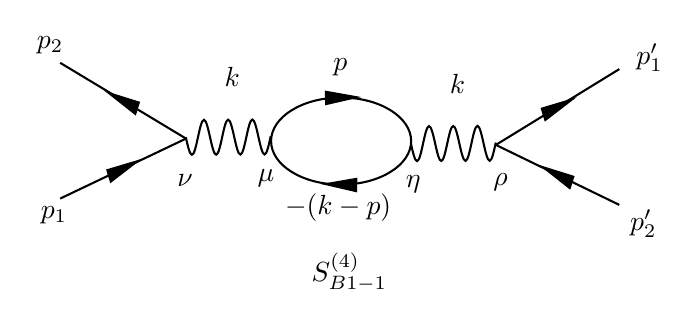
\begin{tikzpicture}[x=0.75pt,y=0.75pt,yscale=-1,xscale=1]
%uncomment if require: \path (0,154); %set diagram left start at 0, and has height of 154

%Straight Lines [id:da05138423204991027] 
\draw    (180.87,29.02) -- (241.51,65.53) ;
%Straight Lines [id:da9811036025098181] 
\draw    (241.51,65.53) -- (180.87,94.43) ;
%Shape: Wave [id:dp737168525141477] 
\draw   (241.41,64.94) .. controls (242.38,69.24) and (243.3,73.34) .. (244.36,73.33) .. controls (245.41,73.33) and (246.31,69.22) .. (247.24,64.91) .. controls (248.18,60.6) and (249.08,56.5) .. (250.13,56.49) .. controls (251.19,56.49) and (252.11,60.58) .. (253.08,64.88) .. controls (254.04,69.18) and (254.96,73.28) .. (256.02,73.27) .. controls (257.07,73.26) and (257.97,69.16) .. (258.91,64.85) .. controls (259.84,60.54) and (260.74,56.44) .. (261.79,56.43) .. controls (262.85,56.43) and (263.77,60.52) .. (264.74,64.82) .. controls (265.7,69.12) and (266.62,73.21) .. (267.68,73.21) .. controls (268.73,73.2) and (269.63,69.1) .. (270.57,64.79) .. controls (271.5,60.48) and (272.4,56.38) .. (273.46,56.37) .. controls (274.51,56.36) and (275.43,60.46) .. (276.4,64.76) .. controls (277.36,69.06) and (278.28,73.15) .. (279.34,73.15) .. controls (280.39,73.14) and (281.29,69.04) .. (282.23,64.73) .. controls (282.25,64.63) and (282.27,64.52) .. (282.3,64.42) ;
%Shape: Ellipse [id:dp6501484350215895] 
\draw   (282.48,66.72) .. controls (282.48,55.14) and (297.58,45.75) .. (316.22,45.75) .. controls (334.85,45.75) and (349.96,55.14) .. (349.96,66.72) .. controls (349.96,78.3) and (334.85,87.69) .. (316.22,87.69) .. controls (297.58,87.69) and (282.48,78.3) .. (282.48,66.72) -- cycle ;
%Shape: Wave [id:dp6960457234841549] 
\draw   (349.87,67.98) .. controls (350.83,72.29) and (351.75,76.38) .. (352.81,76.37) .. controls (353.86,76.37) and (354.76,72.26) .. (355.7,67.95) .. controls (356.63,63.64) and (357.53,59.54) .. (358.59,59.53) .. controls (359.64,59.53) and (360.56,63.62) .. (361.53,67.92) .. controls (362.49,72.22) and (363.41,76.32) .. (364.47,76.31) .. controls (365.53,76.31) and (366.42,72.2) .. (367.36,67.89) .. controls (368.3,63.58) and (369.19,59.48) .. (370.25,59.47) .. controls (371.3,59.47) and (372.23,63.56) .. (373.19,67.86) .. controls (374.15,72.16) and (375.08,76.26) .. (376.13,76.25) .. controls (377.19,76.25) and (378.08,72.14) .. (379.02,67.83) .. controls (379.96,63.52) and (380.85,59.42) .. (381.91,59.41) .. controls (382.96,59.41) and (383.89,63.5) .. (384.85,67.8) .. controls (385.82,72.1) and (386.74,76.2) .. (387.79,76.19) .. controls (388.85,76.18) and (389.74,72.08) .. (390.68,67.77) .. controls (390.7,67.67) and (390.73,67.57) .. (390.75,67.46) ;
%Straight Lines [id:da6531384244314116] 
\draw    (450.25,32.06) -- (390.78,68.57) ;
%Straight Lines [id:da6679889830399947] 
\draw    (390.78,68.57) -- (450.25,97.47) ;
%Shape: Triangle [id:dp22407102566991655] 
\draw  [fill={rgb, 255:red, 0; green, 0; blue, 0 }  ,fill opacity=1 ] (204.48,43.68) -- (218.75,48.15) -- (217.04,53.59) -- cycle ;
%Shape: Triangle [id:dp2670818642470857] 
\draw  [fill={rgb, 255:red, 0; green, 0; blue, 0 }  ,fill opacity=1 ] (413.81,79.43) -- (428.08,83.89) -- (426.36,89.33) -- cycle ;
%Shape: Triangle [id:dp04965090912992787] 
\draw  [fill={rgb, 255:red, 0; green, 0; blue, 0 }  ,fill opacity=1 ] (217.92,76.48) -- (205.28,86.21) -- (203.62,80.74) -- cycle ;
%Shape: Triangle [id:dp8503295318751536] 
\draw  [fill={rgb, 255:red, 0; green, 0; blue, 0 }  ,fill opacity=1 ] (427.25,46.82) -- (414.61,56.54) -- (412.94,51.08) -- cycle ;
%Shape: Triangle [id:dp7966952976838977] 
\draw  [fill={rgb, 255:red, 0; green, 0; blue, 0 }  ,fill opacity=1 ] (323.47,45.57) -- (309.01,48.88) -- (308.93,42.99) -- cycle ;
%Shape: Triangle [id:dp32055391743711603] 
\draw  [fill={rgb, 255:red, 0; green, 0; blue, 0 }  ,fill opacity=1 ] (308.97,87.48) -- (323.52,84.95) -- (323.42,90.83) -- cycle ;

% Text Node
\draw (263.82,35.96) node    {$k$};
% Text Node
\draw (372.27,39.01) node    {$k$};
% Text Node
\draw (320.23,130.1) node    {$S^{( 4)}_{B1-1}$};
% Text Node
\draw (241,85.7) node    {$\nu $};
% Text Node
\draw (280,84.7) node    {$\mu $};
% Text Node
\draw (351,87.7) node    {$\eta $};
% Text Node
\draw (393,86.7) node    {$\rho $};
% Text Node
\draw (315.82,30.96) node    {$p$};
% Text Node
\draw (314.82,98.96) node    {$-( k-p)$};
% Text Node
\draw (176,20.7) node    {$p_{2}$};
% Text Node
\draw (177.87,102.43) node    {$p_{1}$};
% Text Node
\draw (464.87,26.43) node    {$p^{\prime }_{1}$};
% Text Node
\draw (461.87,106.43) node    {$p^{\prime }_{2}$};


\end{tikzpicture}

    \caption{$S^{(4)}_{B1-1}$ term Feynman diagram for Bhabha Scattering}
    \label{fig:SB1-1(4)}
\end{figure}
The Feynman amplitude for this is
\begin{equation}
\frac{-p^{4}}{(2 x)^{4}} \bar{u}_{\eta}^{\prime}\left(\mathbf{p}_{1}^{\prime}\right) \gamma^{\rho} v_{r_{2}^{\prime}}\left(\mathbf{p}_{2}^{\prime}\right) D_{F \rho \eta}(k)\left\{\operatorname{Tr} \int S_{F}(p-k) \gamma^{\eta} S_{F}(p) \gamma^{\mu} d^{4} p\right\}D_{F \mu \nu}(k) \bar{v}_{\tau_{2}}\left(\mathbf{p}_{2}\right) \gamma^{v} u_{r_1}\left(\mathbf{p}_{1}\right)
\label{SB1-1(4)}
\end{equation}
Every momentum value in (\ref{SB1-1(4)}) is fixed except $p$, which must be integrated over 4D momentum space from $+\infty$ to $-\infty$ along all four axes. And we know all of the factors are finite except for the integral. Let's estimate the integral value by \bluep{assuming parts of the integral where any component $p^{\mu}$ is large could be the problematic portions.} That is, we'll specifically investigate whether the integral blows up for large values of $p^{\mu}$.
$$
\int S_{F}(p) \gamma^{\mu} S_{F}(p-k) \gamma^{\eta} d^{4} p=\int \frac{\cancel{p}+m}{p^{2}-m^{2}+i \varepsilon} \gamma^{\mu}\frac{\cancel{p}-\cancel{k}+m}{(p-k)^{2}-m^{2}+i \varepsilon} \gamma^{\eta} d^{4} p
$$
$$\frac{\text { for contribution }}{\text { from large } p}\rightarrow \approx\int \frac{p_{v}}{p^{2}} \gamma^{v} \gamma^{\mu} \gamma^{\sigma} \gamma^{\eta} \frac{p_{\sigma}}{p^{2}} d^{4} p\overset{\text{ignore }\gamma\text{ matrices}}{\Arrow{3.5cm}}\int \frac{p p}{p^{4}} d^{4} p
$$
Since
$$
d A=d^{2} r=2 \pi r d r\quad d V=d^{3} r=4 \pi r^{2} d r\quad d R_{4 D}=d^{4} r=2 \pi^{2} r^{3} \quad d r
$$
Applying the last expression, we have
$$
\int_{-\infty}^{\infty} \frac{d^{4} p}{p^{2}}=\int_{0}^{\infty} 2 \pi^{2} \frac{p^{3}}{p^{2}} d p=2 \pi^{2} \int_{0}^{\infty} p d p=\left.\pi^{2} p^{2}\right|_{0} ^{\infty}
$$
which diverges with the square of $p$ as $p$ gets large, and is called \redp{\textbf{quadratically divergent}}. This procedure of estimating the degree of divergence is called \textbf{power counting, naive power counting, or superficial power counting}. It is called naive/superficial because, as we will see in later chapters, the actual degree of divergence can be less than this estimate. \bluep{Power counting tells us the maximum degree of divergence an integral may have}. For example, the photon loop actually diverges with the log of $p$ at high $p$. More on this later.

\redp{Whenever we have a photon loop, in any scattering case, we will get a factor of infinity in our transition amplitude. Naive power counting indicates the divergence may be proportional to $p^2$, for large memontum.}

\begin{figure}[H]
    \centering
\tikzset{every picture/.style={line width=0.75pt}} %set default line width to 0.75pt        

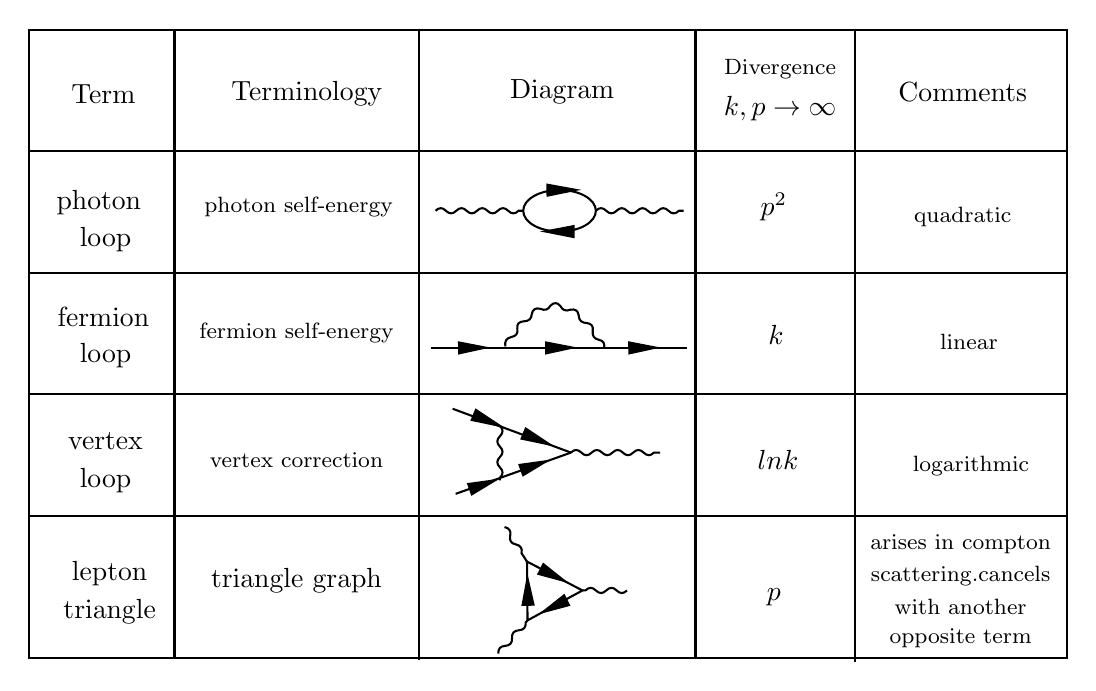
\begin{tikzpicture}[x=0.75pt,y=0.75pt,yscale=-1,xscale=1]
%uncomment if require: \path (0,454); %set diagram left start at 0, and has height of 454

%Shape: Rectangle [id:dp031140315854360834] 
\draw   (71,32) -- (571.25,32) -- (571.25,90.57) -- (71,90.57) -- cycle ;
%Shape: Rectangle [id:dp4895781002142545] 
\draw   (71,90.57) -- (571.25,90.57) -- (571.25,149.13) -- (71,149.13) -- cycle ;
%Shape: Rectangle [id:dp8535986584003854] 
\draw   (71,149.13) -- (571.25,149.13) -- (571.25,207.7) -- (71,207.7) -- cycle ;
%Shape: Rectangle [id:dp6484610804595969] 
\draw   (71,207.7) -- (571.25,207.7) -- (571.25,266.27) -- (71,266.27) -- cycle ;
%Shape: Rectangle [id:dp3458613670457761] 
\draw   (71,266.27) -- (571.25,266.27) -- (571.25,334.67) -- (71,334.67) -- cycle ;
%Straight Lines [id:da612608268750112] 
\draw    (141.25,32.57) -- (141.25,334.67) ;
%Straight Lines [id:da23824933707218732] 
\draw    (259.25,31.57) -- (259.25,335.67) ;
%Straight Lines [id:da04568411553174856] 
\draw    (392.25,32.57) -- (392.25,334.67) ;
%Straight Lines [id:da1154509245060571] 
\draw    (469.25,31.57) -- (469.25,336.67) ;
%Straight Lines [id:da6493776523677909] 
\draw    (267,119.28) .. controls (268.67,117.61) and (270.33,117.61) .. (272,119.28) .. controls (273.67,120.95) and (275.33,120.95) .. (277,119.28) .. controls (278.67,117.61) and (280.33,117.61) .. (282,119.28) .. controls (283.67,120.95) and (285.33,120.95) .. (287,119.28) .. controls (288.67,117.61) and (290.33,117.61) .. (292,119.28) .. controls (293.67,120.95) and (295.33,120.95) .. (297,119.28) .. controls (298.67,117.61) and (300.33,117.61) .. (302,119.28) .. controls (303.67,120.95) and (305.33,120.95) .. (307,119.28) -- (309.25,119.28) -- (309.25,119.28) ;
%Shape: Ellipse [id:dp4946043612693545] 
\draw   (309.25,119.28) .. controls (309.25,113.76) and (317.09,109.28) .. (326.75,109.28) .. controls (336.41,109.28) and (344.25,113.76) .. (344.25,119.28) .. controls (344.25,124.81) and (336.41,129.28) .. (326.75,129.28) .. controls (317.09,129.28) and (309.25,124.81) .. (309.25,119.28) -- cycle ;
%Straight Lines [id:da5015190253711108] 
\draw    (344.25,119.28) .. controls (345.92,117.61) and (347.58,117.61) .. (349.25,119.28) .. controls (350.92,120.95) and (352.58,120.95) .. (354.25,119.28) .. controls (355.92,117.61) and (357.58,117.61) .. (359.25,119.28) .. controls (360.92,120.95) and (362.58,120.95) .. (364.25,119.28) .. controls (365.92,117.61) and (367.58,117.61) .. (369.25,119.28) .. controls (370.92,120.95) and (372.58,120.95) .. (374.25,119.28) .. controls (375.92,117.61) and (377.58,117.61) .. (379.25,119.28) .. controls (380.92,120.95) and (382.58,120.95) .. (384.25,119.28) -- (386.5,119.28) -- (386.5,119.28) ;
%Shape: Triangle [id:dp09740187309204174] 
\draw  [fill={rgb, 255:red, 0; green, 0; blue, 0 }  ,fill opacity=1 ] (334.56,109.21) -- (320.97,111.98) -- (320.91,106.73) -- cycle ;
%Shape: Triangle [id:dp5845786969302623] 
\draw  [fill={rgb, 255:red, 0; green, 0; blue, 0 }  ,fill opacity=1 ] (319.94,129.26) -- (333.57,126.68) -- (333.55,131.93) -- cycle ;
%Straight Lines [id:da6040536328741318] 
\draw    (265,185.28) -- (388.25,185.28) ;
%Shape: Triangle [id:dp6560823900329256] 
\draw  [fill={rgb, 255:red, 0; green, 0; blue, 0 }  ,fill opacity=1 ] (332.97,185.21) -- (320.31,187.98) -- (320.25,182.74) -- cycle ;
%Shape: Triangle [id:dp5836695385624332] 
\draw  [fill={rgb, 255:red, 0; green, 0; blue, 0 }  ,fill opacity=1 ] (373.04,185.21) -- (360.38,187.98) -- (360.33,182.74) -- cycle ;
%Shape: Triangle [id:dp6381006926349475] 
\draw  [fill={rgb, 255:red, 0; green, 0; blue, 0 }  ,fill opacity=1 ] (291.03,185.21) -- (278.37,187.98) -- (278.32,182.74) -- cycle ;
%Curve Lines [id:da7920805686673805] 
\draw    (300.65,184.67) .. controls (300.19,182.21) and (301.14,180.69) .. (303.51,180.11) .. controls (305.82,179.72) and (306.78,178.4) .. (306.39,176.15) .. controls (306.09,173.9) and (307.13,172.69) .. (309.52,172.54) .. controls (311.92,172.53) and (313.21,171.37) .. (313.39,169.06) .. controls (313.8,166.75) and (315.17,165.91) .. (317.5,166.52) .. controls (319.61,167.49) and (321.22,166.99) .. (322.35,165.04) .. controls (324.01,163.29) and (325.62,163.34) .. (327.17,165.19) .. controls (328.19,167.21) and (329.78,167.8) .. (331.95,166.96) .. controls (334.33,166.47) and (335.67,167.39) .. (335.98,169.72) .. controls (336.07,172.04) and (337.32,173.25) .. (339.73,173.36) .. controls (342.11,173.59) and (343.11,174.83) .. (342.73,177.07) .. controls (342.42,179.52) and (343.41,180.98) .. (345.7,181.45) .. controls (347.89,181.84) and (348.71,183.25) .. (348.18,185.67) -- (348.18,185.67) ;
%Straight Lines [id:da16346429830138187] 
\draw    (275.25,214.67) -- (332.25,235.79) ;
%Straight Lines [id:da013119675530554153] 
\draw    (332.25,235.79) -- (276.7,255.67) ;
%Shape: Triangle [id:dp03182221029365928] 
\draw  [fill={rgb, 255:red, 0; green, 0; blue, 0 }  ,fill opacity=1 ] (298.03,222.91) -- (284.46,220.08) -- (286.48,215.23) -- cycle ;
%Shape: Triangle [id:dp1719443782691389] 
\draw  [fill={rgb, 255:red, 0; green, 0; blue, 0 }  ,fill opacity=1 ] (322.03,231.91) -- (308.46,229.08) -- (310.48,224.23) -- cycle ;
%Shape: Triangle [id:dp20847571898296002] 
\draw  [fill={rgb, 255:red, 0; green, 0; blue, 0 }  ,fill opacity=1 ] (295.61,249.17) -- (284.51,255.88) -- (282.77,250.92) -- cycle ;
%Shape: Triangle [id:dp7138372538333491] 
\draw  [fill={rgb, 255:red, 0; green, 0; blue, 0 }  ,fill opacity=1 ] (320.31,239.97) -- (309.22,246.68) -- (307.47,241.73) -- cycle ;
%Straight Lines [id:da023306038639583804] 
\draw    (298.03,222.91) .. controls (299.7,224.58) and (299.7,226.24) .. (298.03,227.91) .. controls (296.36,229.58) and (296.36,231.24) .. (298.03,232.91) .. controls (299.7,234.58) and (299.7,236.24) .. (298.03,237.91) .. controls (296.36,239.58) and (296.36,241.24) .. (298.03,242.91) .. controls (299.7,244.58) and (299.7,246.24) .. (298.03,247.91) -- (298.03,249.17) -- (298.03,249.17) ;
%Straight Lines [id:da1558606395749318] 
\draw    (332.25,235.79) .. controls (333.92,234.12) and (335.58,234.12) .. (337.25,235.79) .. controls (338.92,237.46) and (340.58,237.46) .. (342.25,235.79) .. controls (343.92,234.12) and (345.58,234.12) .. (347.25,235.79) .. controls (348.92,237.46) and (350.58,237.46) .. (352.25,235.79) .. controls (353.92,234.12) and (355.58,234.12) .. (357.25,235.79) .. controls (358.92,237.46) and (360.58,237.46) .. (362.25,235.79) .. controls (363.92,234.12) and (365.58,234.12) .. (367.25,235.79) .. controls (368.92,237.46) and (370.58,237.46) .. (372.25,235.79) -- (375.25,235.79) -- (375.25,235.79) ;
%Shape: Triangle [id:dp6550876901036714] 
\draw   (337.8,302.21) -- (311.33,316.63) -- (311.08,288.29) -- cycle ;
%Straight Lines [id:da9004730431520491] 
\draw    (300.25,271.67) .. controls (302.56,272.16) and (303.47,273.55) .. (302.98,275.86) .. controls (302.49,278.17) and (303.4,279.56) .. (305.71,280.05) .. controls (308.02,280.54) and (308.92,281.93) .. (308.43,284.24) -- (311.07,288.29) -- (311.07,288.29) ;
%Straight Lines [id:da23235660682707382] 
\draw    (359.25,302.21) .. controls (357.58,303.88) and (355.92,303.88) .. (354.25,302.21) .. controls (352.58,300.54) and (350.92,300.54) .. (349.25,302.21) .. controls (347.58,303.88) and (345.92,303.88) .. (344.25,302.21) .. controls (342.58,300.54) and (340.92,300.54) .. (339.25,302.21) -- (337.81,302.21) -- (337.81,302.21) ;
%Straight Lines [id:da01944025161269347] 
\draw    (297.25,332.67) .. controls (297.1,330.32) and (298.2,329.06) .. (300.55,328.91) .. controls (302.9,328.76) and (304,327.5) .. (303.85,325.15) .. controls (303.7,322.8) and (304.8,321.55) .. (307.15,321.4) .. controls (309.5,321.25) and (310.6,319.99) .. (310.45,317.64) -- (311.33,316.63) -- (311.33,316.63) ;
%Shape: Triangle [id:dp4897212554831919] 
\draw  [fill={rgb, 255:red, 0; green, 0; blue, 0 }  ,fill opacity=1 ] (329.1,297.63) -- (316.59,294.24) -- (318.97,289.56) -- cycle ;
%Shape: Triangle [id:dp603613879599554] 
\draw  [fill={rgb, 255:red, 0; green, 0; blue, 0 }  ,fill opacity=1 ] (318.77,312.61) -- (328.94,304.57) -- (331.29,309.27) -- cycle ;
%Shape: Triangle [id:dp7966469483195274] 
\draw  [fill={rgb, 255:red, 0; green, 0; blue, 0 }  ,fill opacity=1 ] (311.3,296.42) -- (314.21,309.06) -- (308.96,309.16) -- cycle ;

% Text Node
\draw (107,63) node   [align=left] {Term};
% Text Node
\draw (205,63) node   [align=left] {Terminology};
% Text Node
\draw (328,62) node   [align=left] {Diagram};
% Text Node
\draw (433,51) node  [font=\footnotesize] [align=left] {Divergence};
% Text Node
\draw (433,70.28) node    {$k,p\rightarrow \infty $};
% Text Node
\draw (521,62.28) node   [align=left] {Comments};
% Text Node
\draw (107,115.28) node [align=center]  {
photon
};
% Text Node
\draw (107,170.28) node  {
fermion
};
% Text Node
\draw (108,230.28) node  {
vertex
};
% Text Node
\draw (110,294.28) node {
lepton
};
% Text Node
\draw (201,117.28) node  {
{\footnotesize photon self-energy}
};
% Text Node
\draw (200,178.28) node  {
{\footnotesize fermion self-energy}
};
% Text Node
\draw (200,239.28) node  {
{\footnotesize vertex correction}
};
% Text Node
\draw (200,297.28) node  { triangle graph
};
% Text Node
\draw (430,117.28) node    {$p^{2}$};
% Text Node
\draw (431,179.28) node    {$k$};
% Text Node
\draw (432,239.28) node    {$lnk$};
% Text Node
\draw (430,305.28) node    {$p$};
% Text Node
\draw (521,122.28) node  [font=\footnotesize] {
quadratic
};
% Text Node
\draw (524,182.28) node  [font=\footnotesize] {
linear
};
% Text Node
\draw (525,242.28) node  [font=\footnotesize] { logarithmic
};
% Text Node
\draw (520,280.0) node  [font=\footnotesize]  {
arises in compton};
\draw (520,295.0) node  [font=\footnotesize]  {
scattering.cancels};
\draw (520,310.0) node  [font=\footnotesize]  {
with another};
\draw (520,325.0) node  [font=\footnotesize]  {
opposite term};
% Text Node
\draw (108,133.28) node  {
loop
};
% Text Node
\draw (108,189.28) node {
loop

};
% Text Node
\draw (108,249.28) node  {
loop

};
% Text Node
\draw (110,312.28) node   {
triangle
};


\end{tikzpicture}

    \caption{Wholeness Chart on Loop corrections}
    \label{fig:loop-correction-table}
\end{figure}

\section{Other terms}
Consider the $S^{(4)}_{B1-8}$ diagram in Fig.\ref{fig:4-order-contribution-Bhabha}, which we show below with momenta and spacetime labels. \textbf{Note there are no simple loops} in Fig.\ref{fig:S4B1-8}. The term loop in QFT generally refers only to one the three simple loops shown above.
\begin{figure}[H]
    \centering
\tikzset{every picture/.style={line width=0.75pt}} %set default line width to 0.75pt        
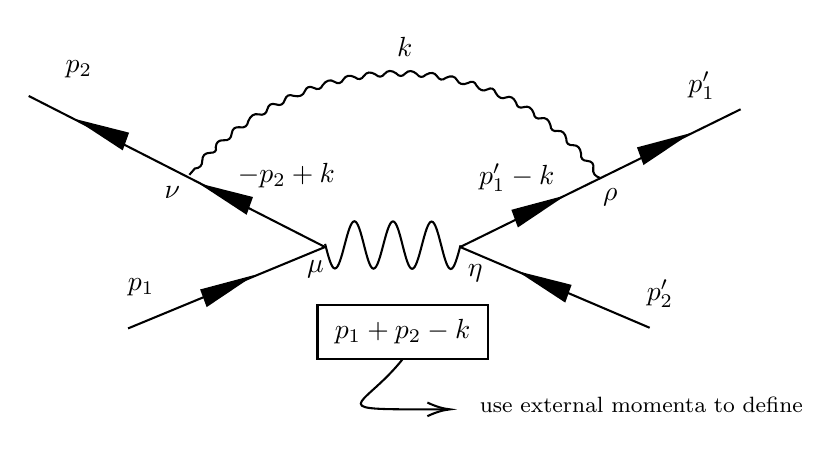
\begin{tikzpicture}[x=0.75pt,y=0.75pt,yscale=-1,xscale=1]
%uncomment if require: \path (0,592); %set diagram left start at 0, and has height of 592

%Straight Lines [id:da04049123588573589] 
\draw    (448.85,408.24) -- (313.73,474.6) ;
%Straight Lines [id:da13254227439928667] 
\draw    (313.73,474.6) -- (405.03,513.51) ;
%Shape: Wave [id:dp19915588527907724] 
\draw   (313.88,473.81) .. controls (312.34,479.64) and (310.87,485.2) .. (309.19,485.19) .. controls (307.51,485.18) and (306.08,479.61) .. (304.58,473.76) .. controls (303.08,467.92) and (301.65,462.35) .. (299.97,462.34) .. controls (298.28,462.33) and (296.81,467.89) .. (295.28,473.72) .. controls (293.74,479.56) and (292.27,485.12) .. (290.59,485.11) .. controls (288.9,485.1) and (287.47,479.53) .. (285.97,473.68) .. controls (284.48,467.83) and (283.05,462.27) .. (281.36,462.26) .. controls (279.68,462.25) and (278.21,467.81) .. (276.67,473.64) .. controls (275.13,479.48) and (273.66,485.04) .. (271.98,485.03) .. controls (270.3,485.02) and (268.86,479.45) .. (267.37,473.6) .. controls (265.87,467.75) and (264.44,462.18) .. (262.76,462.18) .. controls (261.07,462.17) and (259.6,467.73) .. (258.06,473.56) .. controls (256.53,479.4) and (255.06,484.95) .. (253.37,484.95) .. controls (251.69,484.94) and (250.26,479.37) .. (248.76,473.52) .. controls (248.73,473.38) and (248.69,473.24) .. (248.65,473.1) ;
%Straight Lines [id:da3762098971597273] 
\draw    (105.85,401.82) -- (248.61,474.6) ;
%Straight Lines [id:da7653135479566218] 
\draw    (248.61,474.6) -- (153.72,513.82) ;
%Shape: Triangle [id:dp9916239306196007] 
\draw  [fill={rgb, 255:red, 0; green, 0; blue, 0 }  ,fill opacity=1 ] (361.81,450.95) -- (339.05,457.02) -- (341.78,464.4) -- cycle ;
%Shape: Triangle [id:dp8843027624133398] 
\draw  [fill={rgb, 255:red, 0; green, 0; blue, 0 }  ,fill opacity=1 ] (211.86,489.33) -- (189.1,495.4) -- (191.83,502.78) -- cycle ;
%Shape: Triangle [id:dp20733839488922945] 
\draw  [fill={rgb, 255:red, 0; green, 0; blue, 0 }  ,fill opacity=1 ] (343.92,487.4) -- (364.09,500.6) -- (366.75,493.18) -- cycle ;
%Shape: Triangle [id:dp5518194119245399] 
\draw  [fill={rgb, 255:red, 0; green, 0; blue, 0 }  ,fill opacity=1 ] (190.42,445.09) -- (210.58,458.29) -- (213.24,450.87) -- cycle ;
%Shape: Triangle [id:dp9155946701917791] 
\draw  [fill={rgb, 255:red, 0; green, 0; blue, 0 }  ,fill opacity=1 ] (422.34,420.88) -- (399.57,426.94) -- (402.3,434.32) -- cycle ;
%Shape: Triangle [id:dp6087326863588755] 
\draw  [fill={rgb, 255:red, 0; green, 0; blue, 0 }  ,fill opacity=1 ] (130.72,414.06) -- (150.88,427.26) -- (153.54,419.85) -- cycle ;
%Curve Lines [id:da905688656373794] 
\draw    (381.29,441.42) .. controls (378.59,440.51) and (377.44,438.95) .. (377.85,436.72) .. controls (378.2,434.47) and (377.24,433.27) .. (374.97,433.12) .. controls (372.72,433.05) and (371.72,431.89) .. (371.97,429.66) .. controls (371.63,426.84) and (370.33,425.47) .. (368.08,425.54) .. controls (365.85,425.67) and (364.77,424.63) .. (364.84,422.4) .. controls (364.29,419.64) and (362.89,418.4) .. (360.66,418.68) .. controls (358.47,419.02) and (357.32,418.08) .. (357.21,415.87) .. controls (356.44,413.18) and (354.96,412.08) .. (352.78,412.56) .. controls (350.63,413.09) and (349.42,412.26) .. (349.14,410.07) .. controls (348.15,407.48) and (346.6,406.51) .. (344.47,407.18) .. controls (342.38,407.9) and (341.11,407.18) .. (340.65,405.03) .. controls (339.46,402.53) and (337.84,401.7) .. (335.79,402.55) .. controls (333.78,403.45) and (332.12,402.7) .. (330.82,400.31) .. controls (330.09,398.21) and (328.74,397.67) .. (326.77,398.68) .. controls (324.85,399.75) and (323.14,399.14) .. (321.64,396.87) .. controls (320.75,394.84) and (319.36,394.41) .. (317.48,395.59) .. controls (314.97,396.63) and (313.21,396.17) .. (312.22,394.2) .. controls (311.16,392.25) and (309.38,391.87) .. (306.89,393.06) .. controls (305.18,394.44) and (303.74,394.19) .. (302.58,392.32) .. controls (301.36,390.46) and (299.55,390.23) .. (297.16,391.62) .. controls (295.56,393.13) and (294.11,393) .. (292.8,391.23) .. controls (290.68,389.44) and (288.85,389.35) .. (287.31,390.97) .. controls (285.83,392.61) and (284.36,392.6) .. (282.9,390.94) .. controls (280.63,389.33) and (278.78,389.39) .. (277.37,391.12) .. controls (276.02,392.88) and (274.55,392.99) .. (272.94,391.45) .. controls (270.53,390.03) and (268.68,390.24) .. (267.41,392.09) .. controls (266.19,393.96) and (264.71,394.19) .. (262.98,392.79) .. controls (260.43,391.57) and (258.59,391.93) .. (257.45,393.88) .. controls (256.37,395.84) and (254.9,396.19) .. (253.04,394.94) .. controls (251.13,393.73) and (249.3,394.25) .. (247.56,396.5) .. controls (246.62,398.55) and (245.17,399.03) .. (243.2,397.94) .. controls (241.17,396.89) and (239.73,397.43) .. (238.86,399.54) .. controls (238.05,401.65) and (236.26,402.4) .. (233.48,401.77) .. controls (231.35,400.9) and (229.93,401.56) .. (229.22,403.75) .. controls (228.56,405.94) and (227.15,406.65) .. (224.99,405.89) .. controls (222.79,405.19) and (221.4,405.96) .. (220.82,408.21) .. controls (220.29,410.45) and (218.91,411.28) .. (216.68,410.69) .. controls (214.41,410.16) and (212.71,411.28) .. (211.6,414.04) .. controls (211.23,416.34) and (209.89,417.3) .. (207.59,416.91) .. controls (205.25,416.59) and (203.94,417.6) .. (203.65,419.95) .. controls (203.41,422.3) and (202.12,423.37) .. (199.77,423.17) .. controls (197.38,423.04) and (196.11,424.17) .. (195.96,426.56) .. controls (196.47,428.36) and (195.54,429.25) .. (193.15,429.22) .. controls (190.74,429.27) and (189.51,430.5) .. (189.48,432.92) .. controls (189.5,435.33) and (188.3,436.62) .. (185.89,436.79) -- (183.25,439.82) ;
%Curve Lines [id:da24972768989890304] 
\draw    (285.85,528.82) .. controls (266.05,553.57) and (245.27,552.83) .. (306.96,552.82) ;
\draw [shift={(308.85,552.82)}, rotate = 180] [color={rgb, 255:red, 0; green, 0; blue, 0 }  ][line width=0.75]    (10.93,-3.29) .. controls (6.95,-1.4) and (3.31,-0.3) .. (0,0) .. controls (3.31,0.3) and (6.95,1.4) .. (10.93,3.29)   ;

% Text Node
\draw (287,378) node    {$k$};
% Text Node
\draw    (245,502.43) -- (327,502.43) -- (327,528.43) -- (245,528.43) -- cycle  ;
\draw (286,515.43) node    {$p_{1} +p_{2} -k$};
% Text Node
\draw (401,550.43) node  [font=\footnotesize] [align=left] {use external momenta to define};
% Text Node
\draw (341,441) node    {$p^{\prime }_{1} -k$};
% Text Node
\draw (430,397) node    {$p^{\prime }_{1}$};
% Text Node
\draw (410,497) node    {$p^{\prime }_{2}$};
% Text Node
\draw (230,440) node    {$-p_{2} +k$};
% Text Node
\draw (130,389) node    {$p_{2}$};
% Text Node
\draw (160,494) node    {$p_{1}$};
% Text Node
\draw (244,485.43) node    {$\mu $};
% Text Node
\draw (321,487.43) node    {$\eta $};
% Text Node
\draw (386,450.43) node    {$\rho $};
% Text Node
\draw (175,448.43) node    {$\nu $};


\end{tikzpicture}

    \caption{$S_{B1-8}^{(4)}$}
    \label{fig:S4B1-8}
\end{figure}
The Feynman amplitude for the fig above is
$$
\frac{1}{(2 \pi)^{4}} e^{4} \int d^{4} k \bar{u}_{r^{\prime}}\left(\mathbf{p}_{1}^{\prime}\right) \gamma^{\rho} S_{F}\left(p_{1}^{\prime}-k\right) \gamma^{\eta} v_{s^{\prime}}\left(\mathbf{p}_{2}^{\prime}\right) \times
$$
$$
D_{F \eta \mu}\left(p_{1}+p_{2}-k\right) D_{F \rho v}(k)\bar{v}_{s}\left(\mathbf{p}_{2}\right) \gamma^{v} S_{F}\left(-p_{2}+k\right) \gamma^{\mu} u_{r}\left(\mathbf{p}_{1}\right)
$$
Perform naive power counting, we get
$$
\int S_{F}\left(p_{1}^{\prime}-k\right) D_{F}\left(p_{1}+p_{2}-k\right) D_{F}(k) S_{F}\left(-p_{2}+k\right) d^{4} k
$$
$$
\overset{\text{for large} k}{\Arrow{2cm}}\approx \int \frac{1}{k} \frac{1}{k^{2}} \frac{1}{k^{2}} \frac{1}{k} d^{4} k=2 \pi^{2} \int \frac{1}{k^{6}} k^{3} d k=-\pi^{2} \frac{1}{k^{2}}
$$
\bluep{So this Feynman amplitude integral converges in the large $k$ region.} For $k\rightarrow0$, we have
$$
\mathcal{M}_{B1-8}^{(4)}\overset{\text{for small }k}{\Arrow{2cm}}\int \frac{\cancel{p_1^{\prime}}+m}{p_{1}^{\prime 2}-m^{2}+i \varepsilon}\frac{1}{\left(p_{1}+p_{2}\right)^{2}+i \varepsilon}
\frac{1}{k^{2}+i \varepsilon}\frac{-\cancel{p}_{2}+m}{p_{2}^{2}-m^{2}+i \varepsilon} d^{4} k
$$
$$
\approx \int(\text { constant }) \frac{1}{k^{2}} d^{4} k \approx2 \pi^{2} \int \frac{1}{k^{2}} k^{3} d k=\pi^{2} k^{2} \text { for small } k
$$
Hence, the integral is finite.
\begin{qt}
        The photon,electron, and vertex loops would all lead to factors of infinity in the transition amplitude. All other terms would be finite, only the loop factors are unbounded.
        
        High momentum divergences are referred to as \textbf{ultraviolet divergence}, while divergence at small momentum region is called \textbf{infrared divergences}.
\end{qt}

\begin{qt}
\textbf{Tricks for Writing out Feynman Amplitude}

\begin{easylist}
\NewList
@ Before write an amplitude down, label the vertices in Feynman diagram using different greek letters
@ By following the time line, the vertex labels should appear in the expression sequentially
@ For each vertex, always put a $ie\gamma^{\mu}$ between two spinor vectors
@ Always put spinor vector at the left of a gamma matrix, and put its adjoint vector at the right of the matrix
@ If there are multiple virtual particles in a diagram, finish its business at earlier spacetime first then go to the later spacetime.
\end{easylist}
\end{qt}

